%%% packages %%%
%%%%%%%%%%%%%%%%%%%%%%%%%%%%%%%%%%%%%%%%%%%%%%%%%%%%%%%%%%%%%%%%%%%%%%%%%%%%%%%  
\documentclass[frenchb]{report}
%\usepackage{natbib}
\usepackage[toc,page]{appendix}
\usepackage[dvipsnames]{xcolor}
\usepackage[french]{babel}
\usepackage{url}
\usepackage[utf8x]{inputenc}
\usepackage{graphicx}
\graphicspath{{images/}}
\usepackage{parskip}
\usepackage{fancyhdr}
\usepackage{fancyvrb}
\usepackage{vmargin}
\usepackage{xcolor}
\usepackage{bbm}
\usepackage{amsmath,amssymb}
\usepackage{amsthm}
\usepackage{dsfont}
\usepackage{stmaryrd}
\usepackage{systeme}
\usepackage{enumitem}
\usepackage{xcolor}
\usepackage{pifont}
\usepackage{textcomp}
\usepackage{calrsfs}
\usepackage[T1]{fontenc}
\usepackage[toc,page]{appendix}
\usepackage{lipsum}
\usepackage{verbatim}
\usepackage{listings}
\usepackage{adforn}
\usepackage{float}
% Les packages necessaires pour faire le pseudo code
%%%%%%%%%%%%%%%%%%%%%%%%%
\usepackage{algorithm}
\usepackage{algorithmic}
%%%%%%%%%%%%%%%%%%%%%%%%%
% Je renomme les commandes en français
%%%%%%%%%%%%%%%%%%%%%%%%%%%%%%%%%%%%%%%%%%%%%%%%%%%%%%%%%%%%%%%
\renewcommand{\algorithmicrequire}{\textbf{Entrée(s) :}}
\renewcommand{\algorithmicreturn}{\textbf{retourner}}
\renewcommand{\algorithmicensure}{\textbf{Initialisation ;}}
\renewcommand{\algorithmicwhile}{\textbf{Tant que}}
\renewcommand{\algorithmicdo}{\textbf{Initialisation}}
\renewcommand{\algorithmicendwhile}{\textbf{fin du Tant que ;}}
\renewcommand{\algorithmicend}{\textbf{fin}}
\renewcommand{\algorithmicif}{\textbf{si}}
\renewcommand{\algorithmicendif}{\textbf{fin du si}}
\renewcommand{\algorithmicelse}{\textbf{sinon}}
\renewcommand{\algorithmicelsif}{\textbf{fin du sinon}}
\renewcommand{\algorithmicthen}{\textbf{alors}}
\renewcommand{\algorithmicthen}{\textbf{Étape E}}
\renewcommand{\algorithmicthen}{\textbf{Étape M}}
\renewcommand{\algorithmicfor}{\textbf{pour}}
\renewcommand{\algorithmicforall}{\textbf{pour tout}}
\renewcommand{\algorithmicto}{\textbf{à}}
\renewcommand{\algorithmicendfor}{\textbf{fin du pour}}
\renewcommand{\algorithmicdo}{\textbf{faire}}
\renewcommand{\algorithmicloop}{\textbf{boucler}}
\renewcommand{\algorithmicendloop}{\textbf{fin de la boucle}}
\renewcommand{\algorithmicrepeat}{\textbf{répéter}}
\renewcommand{\algorithmicuntil}{\textbf{jusqu’à}}
%%%%%%%%%%%%%%%%%%%%%%%%%%%%%%%%%%%%%%%%%%%%%%%%%%%%%%%%%%%%%%%
\setlength{\hoffset}{-18pt}        
\setlength{\oddsidemargin}{0pt} % Marge gauche sur pages impaires
\setlength{\evensidemargin}{9pt} % Marge gauche sur pages paires
\setlength{\marginparwidth}{54pt} % Largeur de note dans la marge
\setlength{\textwidth}{481pt} % Largeur de la zone de texte (17cm)
\setlength{\voffset}{-18pt} % Bon pour DOS
\setlength{\marginparsep}{7pt} % Séparation de la marge
\setlength{\topmargin}{0pt} % Pas de marge en haut
\setlength{\headheight}{13pt} % Haut de page
\setlength{\headsep}{10pt} % Entre le haut de page et le texte
\setlength{\footskip}{27pt} % Bas de page + séparation
\setlength{\textheight}{708pt} % Hauteur de la zone de texte (25cm)
\usepackage{hyperref}
\lstset{%
            inputencoding=utf8,
                extendedchars=true,
                literate=%
                {é}{{\'e}}{1}%
                {è}{{\`e}}{1}%
                {à}{{\`a}}{1}%
                {ç}{{\c{c}}}{1}%
                {œ}{{\oe}}{1}%
                {ù}{{\`u}}{1}%
                {É}{{\'E}}{1}%
                {È}{{\`E}}{1}%
                {À}{{\`A}}{1}%
                {Ç}{{\c{C}}}{1}%
                {Œ}{{\OE}}{1}%
                {Ê}{{\^E}}{1}%
                {ê}{{\^e}}{1}%
                {î}{{\^i}}{1}%
                {ô}{{\^o}}{1}%
                {û}{{\^u}}{1}%
                {ë}{{\¨{e}}}1
                {û}{{\^{u}}}1
                {â}{{\^{a}}}1
                {Â}{{\^{A}}}1
                {Î}{{\^{I}}}1
        }
    
    
\lstset{language=R,
  backgroundcolor=\color{lightgray},   % choose the background color; you must add \usepackage{color} or \usepackage{xcolor}; should come as last argument %MidnightBlue
   basicstyle=\small\ttfamily\color{white},        % the size of the fonts that are used for the code
  breakatwhitespace=false,         % sets if automatic breaks should only happen at whitespace
  breaklines=true,                 % sets automatic line breaking
  captionpos=b,                    % sets the caption-position to bottom
  commentstyle=\color{SpringGreen},    % comment style
  deletekeywords={data,frame,length,as,character},           % if you want to delete keywords from the given language
  extendedchars=true,              % lets you use non-ASCII characters; for 8-bits encodings only, does not work with UTF-8
  frame=single,	                   % adds a frame around the code
  keepspaces=true,                 % keeps spaces in text, useful for keeping indentation of code (possibly needs columns=flexible)
   keywordstyle=\color{Peach},       % keyword style
  morekeywords={kable,*,...},            % if you want to add more keywords to the set
  numbers=left,                    % where to put the line-numbers; possible values are (none, left, right)
  numbersep=5pt,                   % how far the line-numbers are from the code
  %numberstyle=\tiny\color{gray}, % the style that is used for the line-numbers
  rulecolor=\color{white},         % if not set, the frame-color may be changed on line-breaks within not-black text (e.g. comments (green here))
  showspaces=false,                % show spaces everywhere adding particular underscores; it overrides 'showstringspaces'
  showstringspaces=false,          % underline spaces within strings only
  showtabs=false,                  % show tabs within strings adding particular underscores
  stepnumber=2,                    % the step between two line-numbers. If it's 1, each line will be numbered
      % string literal style
  tabsize=2,	                   % sets default tabsize to 2 spaces
  title=\lstname,                  % show the filename of files included with \lstinputlisting; also try caption instead of title
  mathescape=true,
  escapechar=|
  }
%%%%%%%%%%%%%%%%%%%%%%%%%%%%%%%%%%%%%%%%%%%%%%%%%%%%%%%%%%%%%%%%%%%%%%%%%%%%%%%        


        
\makeatletter
\let\thetitle\@title
\let\theauthor\@author
\let\thedate\@date
\makeatother

%%% commandes mise en page %%%
%%%%%%%%%%%%%%%%%%%%%%%%%%%%%%%%%%%%%%%%%%%%%%%%%%%%%%%%%%%%%%%%%%%%%%%%%%%%%%%        
\newcommand{\ld}{\log_{2}}
\newcommand{\R}{\mathbbm{R}}
\newcommand{\N}{\mathbbm{N}}
\newcommand{\1}{\mathbbm{1}}
\newcommand{\E}{\mathbbm{E}}
\newcommand{\V}{\mathbbm{V}}
\newcommand{\prob}{\mathbbm{P}}
\newcommand{\Nc}{\mathcal{N}}
\newcommand{\Cc}{\mathcal{C}}
\newcommand{\K}{\mathcal{K}}
\newcommand{\Xti}{\widetilde{X_i}}
\newcommand{\Xtj}{\widetilde{X_j}}
\newcommand{\Xn}{\overline{X_n}}
\newcommand{\gn}{\hat{g_n}}
\newcommand{\n}{\mathcal{N}}
\newcommand{\lv}{\mathcal{L}}
\newcommand{\thetat}{\tilde{\theta}}

\newcommand{\console}[1]{\colorbox{black}{\begin{minipage}[c]{1\linewidth}\textcolor{white}{\texttt{#1}}\end{minipage}}}

\newtheorem{prop}{Proposition}
\newtheorem{thm}{Théorème}
\newtheorem{cor}{Corollaire}
\newtheorem{lem}{Lemme}
\newtheorem{hyp}{Hypothèse}
\theoremstyle{definition}\newtheorem{defn}{Définition}
\theoremstyle{definition}\newtheorem{exm}{Exemple}
\theoremstyle{definition}\newtheorem{nota}{Notation}
\theoremstyle{definition}\newtheorem{rem}{Remarque}

\renewcommand{\qedsymbol}{\adfhangingflatleafright}


\begin{document}
%%% Pour l'annexe
\def\appendixpage{\vspace*{8cm}
\begin{center}
\Huge\textbf{Annexes}
\end{center}
}
\def\appendixname{Annexe}%
%%%

%%% Page de garde %%%
%%%%%%%%%%%%%%%%%%%%%%%%%%%%%%%%%%%%%%%%%%%%%%%%%%%%%%%%%%%%%%%%%%%%%%%%%%%%%%%%%%%%%%%%%
\begin{titlepage}
\begin{center}

\includegraphics[scale=0.6]{logo.png}
\hfill

\includegraphics[scale=0.35]{fds_logo.png}\\[3cm]
\linespread{1.2}\huge {\bfseries Projet Master 1 SSD }\\[0.5cm]
\linespread{1.2}\LARGE {\bfseries Un modèle pour les nids d'oiseaux}\\[1.5cm]
\linespread{1}

{\large Rédigé par\\}
{\Large \textsc{carvaillo} Thomas}\\
{\Large \textsc{côme} Olivier}\\
{\Large \textsc{pralon} Nicolas}\\[1cm]
{\large \emph{Encadrante :} Elodie \textsc{Brunel-Piccinini}}\\[1.5cm] 


\includegraphics[scale=0.7]{imag_logo.png}

\end{center}
\end{titlepage}
%%%%%%%%%%%%%%%%%%%%%%%%%%%%%%%%%%%%%%%%%%%%%%%%%%%%%%%%%%%%%%%%%%%%%%%%%%%%%%%%%%%%%%%%%
\tableofcontents
\newpage
%%%%%%%%%%%%%%%%%%%%%%%%%%%%%%%%%%%%%%%%%%%%%%%%%%%%%%%%%%%%%%%%%%%%%%%%%%%%%%%%%%%%%%%%%

\chapter*{Introduction}
\addcontentsline{toc}{part}{Introduction}
L’observation est une composante essentielle en sciences appliquées, et tout particulièrement pour nous, futur statisticiens. Ces dernières nous permettent d’élaborer des modèles, et dans le cadre de l’estimation paramétrique, de construire des estimateurs.

Dans la situation où les données sont correctement observées, cadre idéal, la statistique inférentielle nous permet d’obtenir d’agréables expressions analytiques des estimateurs, notamment par la méthode du maximum de vraisemblance, qui est d'une redoutable efficacité. Toujours est-il que ces situations sont peu courantes ; nous sommes souvent confrontés à des situations présentant des données « cachées » ou manquantes. Dans ce dernier cas, nous verrons que les méthodes analytiques exactes ne suffisent plus, et qu’il est nécessaire d’introduire de nouvelles méthodes, également 	basées sur le principe du maximum de vraisemblance, pour tenter d’estimer les paramètres.

Nous étudierons dans le présent projet l’une de ces méthodes, conçue par Dempster et al. (1977), l’algorithme Expectation-Maximization.  

Nous nous appuierons sur un exemple extrait de l’ornithologie ; les données observées seront celles des volumes des nids d’oiseaux, et les données manquantes seront l’espèce qui l’a construit.

Dans un premier chapitre, nous modéliserons mathématiquement le problème et poserons les bases théoriques nécessaires à l’étude; nous verrons brièvement le cas des données complètes, puis étudierons le cas des observations manquantes. Une second chapitre sera consacré à une description et une implémentation en langage $R$ de l’algorithme EM. Puis, dans un troisième chapitre, nous étudierons les performances des résultats ce notre implémentation à l'aide de simulation; nous détaillerons notre implémentation, et étudierons son risque d'erreur. Dans un quatitème et dernièr chapitre, nous considererons une suite d'observations, et proposerons une étude de cas à l'aide des outils que nous aurons implémenté.

\pagebreak
%%%%%%%%%%%%%%%%%%%%%%%%%%%%%%%%%%%%%%%%%%%%%%%%%%%%%%%%%%%%%%%%%%%%%%%%%%%%%%%%%%%%


%%% Premier chapitre %%%
\chapter{Modélisation du problème et liminaire mathématique}
Dans ce premier chapitre, nous introduirons les outils nécessaires pour modéliser mathématiquement le problème. Puis, nous présenterons successivement les deux situations existantes dans le cadre du recueil de données des nids d'oiseaux : celle dans laquelle et l'espèce et la volume du nid ont été observés; et celle dans laquelle seule le volume a pu être observé.
Nous verrons et ce qui diffère entre ces deux situations, et les raisons qui ont incité à la création de l’algorithme EM, l’objet de notre projet. 

Ce chapitre s'inspirera des références [1], [2] et [3]

% section 1
\section{Modélisation du problème}

Nous allons pour commencer donner une première définition, qui est au coeur du présent projet.

\begin{defn}[Loi de mélange]
On appelle loi de mélange toute loi dont la densité s'écrit sous la forme d'une combinaison convexe de plusieurs densités. Si l'on se donne $J$  densités $f_1(x), \cdots, f_J(x)$, alors toute variable aléatoire $X$ dont la densité $f$ s'exprime, pour tout $x\in\R$, sous la forme
\begin{center}
$f(x) := \displaystyle\sum_{i=1}^J \alpha_i f_i(x)$ , $\alpha_i \in\R_+^*$ et $\displaystyle\sum_{j=1}^J\alpha_j=1$ \end{center}
suit une loi de mélange.
\end{defn}

Afin de modéliser commodément le problème, nous introduisons les variables aléatoires suivantes :

\begin{itemize}[label=\adfflowerleft]
	\item La variable aléatoire $X$, modélisant le volume des nids, de densité $f$
	\item $Z$, la variable aléatoire discrète et à valeurs dans $\llbracket 1,J\rrbracket$, représentant l'espèce d'oiseau qui a construit le nid
\end{itemize}

Enfin, nous nous placerons sous les hypothèses suivantes:

\begin{hyp}
Nous supposerons que, $\forall j\in \llbracket 1,J \rrbracket$, la taille des nids d'une espèce $j$ ( \underline{i.e.} $X$ conditionnellement à $(Z=j)$ ) suit une loi normale $\n(\mu_j,v_j)$. Nous dénoterons par $f(x | Z = j) := \gamma_{\mu_j, v_j}(x)$ cette densité.
\end{hyp}


\begin{hyp}
Soit $\Theta := \{ \theta = (\alpha_j,\mu_j, v_j)_{1 \leq j \leq J} \text{ tels que } \alpha_j > 0 \text{ } \forall j\in \llbracket 1,J\rrbracket \text{ et } \displaystyle\sum_{j=1}^J\alpha_j=1\}$. Soient $X_1, \cdots, X_n$ un échantillon de même loi que $X$. On supposera qu'il existe un $\theta \in \Theta$ tel que les données récoltées, ici les tailles des nids, soient la réalisation du précédent échantillon.
\end{hyp}

\begin{rem}
La variable $Z$ est discrète et à valeur dans un sous-ensemble fini de $\N$, elle suit donc une loi 
\begin{center} $\displaystyle \sum_{j=1}^J \alpha_j\delta_j$ \end{center}
\underline{où} $J$ représente le nombre d'espèce de d'oiseaux considéré et les $\alpha_j$ sont des réels, positifs stricts, représentant la proportion de nids de l'espèce $j$, tels que $\displaystyle\sum_{i=1}^J \alpha_j = 1$.
\end{rem}

Il s'ensuit la proposition suivante, qui sera essentielle dans la suite.
\begin{prop}
La distribution de la taille des nids des oiseaux, \underline{i.e.} $X$, admet pour densité ,au point $x$ et par rapport à la mesure de Lebesgue sur $\R$, la fonction $f_ \theta$ définie comme suit
\begin{center} $f_\theta(x) = \displaystyle\sum_{j=1}^J \alpha_j \gamma_{\mu_j, v_j}(x) $ \end{center}
\end{prop}

\begin{proof}
En effet, 
\begin{align*}
\prob(X\leq x) &= \prob\left(\bigcup_{j=1}^J (X\leq x)\cap(Z=j)\right)\\
&=\displaystyle\sum_{j=1}^J \prob((X\leq x)\cap(Z=j))\\
&=\displaystyle\sum_{i=1}^J\prob(Z=j)\times\prob(x\leq X | Z = j) \\
&=\displaystyle\sum_{i=1}^J\alpha_i\times\prob(x\leq X | Z = j) \\
&=\displaystyle\sum_{i=1}^J\alpha_i\times f(x| Z = j) \\
\end{align*}

\end{proof}

Le but de ce projet sera d'étudier des méthodes permettant l'estimation des divers paramètres de cette densité. Nous dénoterons par $\theta := (\alpha_j, \mu_j, v_j)_{1\leq j\leq J}$ le vecteur des paramètres.

\section{Une histoire de densités}

Introduisons une dernière densité et une dernière probabilité, qui nous seront fort utile dans la suite : 

\begin{prop} Nous avons les résultats suivant :
\begin{enumerate}
\item La loi du couple $(X,Z)$ est donnée par 
\begin{align*} 
\prob(X\leq x, Z = j) &= \displaystyle\int_{-\infty}^x f_\theta(u | Z = j)\times\prob(Z=j)du\\
&= \displaystyle\int_{-\infty}^x  \underbrace{\gamma_{\mu_j, v_j}(u) \times \alpha_j }_{:= h_\theta(u,j)}du
\end{align*}
\underline{où} $h_\theta(u,j)$ est la "sous-densité" de $X\times\1_{(Z=j)}$
\item La probabilité de la loi de $Z$ sachant $X=x$ est donnée par:
\begin{center} $\prob_\theta(Z = j | X = x)=\displaystyle \frac{\gamma_{\mu_j, v_j}\times\alpha_j}{f_\theta(x)}$ \end{center}
\underline{où} $f_\theta(x)$ est donnée par la proposition 1.
\end{enumerate}
\end{prop}

\begin{proof}
En effet, 
\begin{align*}
\prob(X\leq x, Z = j) = \displaystyle\int_{-\infty}^x \prob(Z = j | X = u) \times f_\theta(u) du
\end{align*}
On obtient dès lors
\begin{center}
$\prob(Z = j | X = u)\times f_\theta(u) = \gamma_{\mu_j, v_j}(u) \times \alpha_j$
\end{center}
Soit
\begin{center}
$\prob(Z = j | X = u) = \displaystyle\frac{\gamma_{\mu_j, v_j}(u)\times\alpha_j}{f_\theta(u)} := \frac{h_\theta(u,j)}{f_\theta(u)}$
\end{center}
\end{proof}

\begin{rem}
Nous pouvons dès à présent noter que pour un échantillon $X_1, \cdots, X_n$ de même loi que $X$, nous avons 
\begin{center}
$\forall i \in \llbracket 1,n \rrbracket$, $h_\theta(X_i,j) = f_\theta(X_i) \times \prob_\theta(Z = j | X = X_i )$
\end{center}
Ceci nous sera utile dans la suite.
\end{rem}

Nous allons dès à présent nous intéresser à l'estimation de ces paramètres.

% Section 2
\section{Une approche idéaliste}

Regardons dans un premier temps un cas simplifié, un cas ne décrivant pas la réalité des observations mais qui constitue une agréable entrée en matière. \newline
Nous supposerons ici qu'ont été relevés simultanément et les mesures des tailles des nids et l'espèce d'oiseau qui l'a construit. Les observations considérées ici sont donc composées des couples $(X_i, Z_i)$, $i \in \llbracket1,n \rrbracket$. On considérera dès lors la fonction de densité $h_\theta(x,z)$, donnée par la proposition 2. \newline
L'estimation des divers paramètres est alors élémentaire, en témoigne les propositions suivantes :
\begin{prop}[Fonction de Log-vraisemblance]
La Log-vraisemblance du modèle s'écrit
\begin{center} $\mathcal{L}_\theta(X_1, \cdots, X_n, Z_1, \cdots, Z_n) = \displaystyle \sum_{j=1}^J \#A_j ln(\alpha_j) + \sum_{j=1}^J\sum_{i\in A_j}ln(\gamma_{\mu_j, v_j}(X_i))$ \end{center}
\underline{où} les $A_j$ sont définis par $A_j := \{ i\in \llbracket1,n \rrbracket$ tels que $Z_i = j \}$ \underline{i.e.} $\displaystyle\bigcup_{j=1}^J A_j = \llbracket1,n \rrbracket$
\end{prop}
Avant de démontrer cette proposition, nous allons introduire une notation qui nous sera immédiatement utile :
\begin{nota}
Dans ce qui suit, nous noterons
\begin{center}
$\delta_j := \1_{(Z_i = j)}(Z_i)$
\end{center}
Ainsi, 
\begin{center}
$h_\theta(X_i, Z_i) = \displaystyle\prod_{j=1}^J h_\theta(X_i, Z_i)^{\delta_j}$
\end{center}
\end{nota}

\begin{proof}
La Log-vraisemblance du modèle s'écrit:
\begin{align*}
\mathcal{L}_\theta(X_1, \cdots, X_n, Z_1, \cdots, Z_n) 
&= ln\left(\displaystyle\prod_{i=1}^n h_\theta(X_i, Z_i) \right)\\
&= ln\left(\displaystyle\prod_{i=1}^n\prod_{j=1}^J h_\theta(X_i, Z_i)^{\delta_j} \right)\\
&= \1_{(Z_i = j)}(Z_i)\times ln\left(\displaystyle\prod_{i=1}^n\prod_{j=1}^J h_\theta(X_i, Z_i) \right)\\
\end{align*}
$Z_i$ est à valeur dans $j\in\llbracket 1, J \rrbracket$, on  partitionne donc $I := \llbracket1,n \rrbracket$ comme $I = \displaystyle\bigcup_{j=1}^J A_j$. \newline
Ceci va nous permettre de nous désencombrer de l'indicatrice en réindexant la somme. Nous obtenons dès lors : 
\begin{align*}
\mathcal{L}_\theta(X_1, \cdots, X_n, Z_1, \cdots, Z_n) &=  ln\left(\displaystyle\prod_{i\in A_i}\prod_{j=1}^J h_\theta(X_i, Z_i) \right)\\
&= ln\left(\displaystyle\prod_{i\in A_i}\prod_{j=1}^J  \alpha_j\gamma_{\mu_j, v_j}(X_i) \right)\\
&=\displaystyle\sum_{i\in A_i}\sum_{j=1}^J ln(\alpha_{j}\gamma_{\mu_j, v_j}(X_i))\\
&= \displaystyle\sum_{j=1}^J\sum_{i\in A_j} ln(\alpha_j)+ \sum_{j=1}^J\sum_{i\in A_j} ln(\gamma_{\mu_j, v_j}(X_i)) \\
&= \displaystyle\sum_{j=1}^J \#A_j ln(\alpha_j)+ \sum_{j=1}^J\sum_{i\in A_j} ln(\gamma_{\mu_j, v_j}(X_i)) \\
\end{align*}
\end{proof}
Nous pouvons dès lors maximiser la log-vraisemblance afin d'obtenir les estimateurs souhaités :
\begin{prop}[Estimateurs]
Les estimateurs du maximum de vraisemblance $\widehat{\alpha_j}$ (resp. $\widehat{\mu_j}$, et $\widehat{v_j}$) de $\alpha_j$ (resp. $\mu_j$ et $v_j$) sont donnés par
\begin{center}
$\widehat{\alpha_j} = \frac{\#A_j}{n}$
\end{center}
\begin{center}
$ \widehat{\mu_j} = \displaystyle\frac{\sum_{i\in A_j} X_i}{\#A_j} $
\end{center}
\begin{center}
$ \widehat{v_j} = \displaystyle \frac{\sum_{i\in A_j}(X_i - \widehat{\mu_j})^2}{\#A_j}$
\end{center}
\end{prop}

\begin{proof}
Soit $\theta = (\alpha_j, \mu_j, v_j)_{j \in \llbracket 1,J \rrbracket}$. Il s'agit de déterminer 
\begin{center}
	$\underset{\theta\in\R^{3J}, \sum_{j=1}^J\alpha_j = 1}{\text{argmax}}\left(\displaystyle\sum_{j=1}^J \#A_j ln(\alpha_j)+ \sum_{j=1}^J\sum_{i\in A_j} ln(\gamma_{\mu_j, v_j}(X_i))\right)$
\end{center}
Nous avons donc à résoudre un programme de minimisation d'une fonction convexe sur un convexe avec une contraire égalité, il est ainsi naturel de faire appel au Lagrangien. \newline 
Ce dernier s'écrit
\begin{align*} 
L(\theta) &= \displaystyle\sum_{j=1}^J \#A_j ln(\alpha_j)+ \sum_{j=1}^J\sum_{i\in A_j} ln(\gamma_{\mu_j, v_j}(X_i)) - \lambda\times\left(\sum_{j=1}^J\alpha_j - 1\right)\\
&= \displaystyle\sum_{j=1}^J \#A_j ln(\alpha_j)+ \sum_{j=1}^J\sum_{i\in A_j} ln\left(\frac{1}{\sqrt{2\pi v_j}}\exp\left(-\frac{\left(X_i -\mu_j\right)^2}{2v_j} \right)\right) - \lambda\times\left(\sum_{j=1}^J\alpha_j - 1\right)\\
&= \displaystyle\sum_{j=1}^J \#A_j ln(\alpha_j)+ \sum_{j=1}^J\sum_{i\in A_j}\left( \frac{-1}{2}ln(2\pi v_j) -\frac{(X_i-\mu_j)^2}{2v_j}\right) - \lambda\times\left(\sum_{j=1}^J\alpha_j - 1\right)\\
\end{align*}

Il reste maintenant à résoudre le système suivant, afin d'obtenir le vecteur $\widehat{\theta} := (\widehat{\alpha_j}, \widehat{\mu_j}, \widehat{v_j})_{j\in\llbracket 1,J \rrbracket}$ solution du programme.

$
\begin{cases}
\displaystyle\frac{\#A_j}{\widehat{\alpha_j}} - \lambda &= 0 \text{ } \forall j \in \llbracket 1,J \rrbracket \\
\displaystyle\sum_{i\in A_j} (X_i-\widehat{\mu_j})/\widehat{v_j} & = 0 \text{ } \forall j \in \llbracket 1,J \rrbracket \\
\displaystyle\sum_{i\in A_j} \frac{-0.5 \times 2 \times \pi}{2\pi \widehat{v_j}} +\frac{(X_i-\widehat{\mu_j})^2}{2\widehat{v_j}^2} &= 0 \text{ } \forall j \in \llbracket 1,J \rrbracket\\
\displaystyle\sum_{j=1}^J \widehat{\alpha_j} = 1
\end{cases}
$

Ceci équivaut à 

$
\begin{cases}
\displaystyle\frac{\#A_j}{\widehat{\alpha_j}} &= \lambda \text{ } \forall j \in \llbracket 1,J \rrbracket \\
\displaystyle\sum_{i\in A_j}X_i & =\displaystyle\sum_{i\in A_j} \widehat{\mu_j} \text{ } \forall j \in \llbracket 1,J \rrbracket \\
\displaystyle\sum_{i\in A_j} (X_i-\widehat{\mu_j})^2 &= \displaystyle\sum_{i\in A_j} \widehat{v_j}  \text{ } \forall j \in \llbracket 1,J \rrbracket \\
\displaystyle\sum_{j=1}^J \widehat{\alpha_j} = 1
\end{cases}
$
$\Leftrightarrow$
$
\begin{cases}
\displaystyle\frac{\#A_j}{\widehat{\alpha_j}} &= \lambda \text{ } \forall j \in \llbracket 1,J \rrbracket \\
\displaystyle\sum_{i\in A_j}\frac{X_i}{\#A_j} & = \widehat{\mu_j} \text{ } \forall j \in \llbracket 1,J \rrbracket \\
\displaystyle\sum_{i\in A_j} \frac{(X_i-\widehat{\mu_j})^2}{\#A_j} &=  \widehat{v_j}  \text{ } \forall j \in \llbracket 1,J \rrbracket \\
\displaystyle\sum_{j=1}^J \widehat{\alpha_j} = 1
\end{cases}
$

En sommant les $J$ premières lignes du système, on obtient $\displaystyle\sum_{j=1}^J\#A_j = \sum_{j=1}^J\widehat{\alpha_j}\lambda$, \underline{i.e.} $\lambda = n$. En injectant ceci dans le précédent système, on obtient finalement ce qui était annoncé :

$
\begin{cases}
\widehat{\alpha_j} &= \displaystyle \frac{\#A_j}{n} \text{ } \forall j \in \llbracket 1,J \rrbracket \\
\widehat{\mu_j} &= \displaystyle\sum_{i\in A_j}\frac{X_i}{\#A_j} \text{ } \forall j \in \llbracket 1,J \rrbracket \\
\widehat{v_j} &= \displaystyle\sum_{i\in A_j} \frac{(X_i-\widehat{\mu_j})^2}{\#A_j}  \text{ } \forall j \in \llbracket 1,J \rrbracket \\
\end{cases}
$
\end{proof}


%section 3
\section{Une situation concordante à la réalité} % approche réelle // situation naturelle // concordance
Nous nous placerons désormais dans un contexte tout autre que celui du paragraphe précédent, un contexte concordant davantage à la réalité. Dans ce qui suit, nous supposerons que ne sont observées que les tailles des nids, les diverses espèces d'oiseaux les ayant construit étant en quelque sorte des données inobservées ou "cachées". Nous avons donc un échantillon $X_1,\cdots, X_n$ de même loi que la variable $X$ comme définie ci-dessus. \newline
La log-vraisemblance des observations $\mathcal{L}_{obs}$ s'obtient aisément : 
\begin{center} $\mathcal{L}_{obs}(\theta, X_1, \cdots, X_n) := ln\left( \displaystyle\prod_{i=1}^n f_\theta(X_i) \right) = \displaystyle\sum_{i=1}^nln\left( \sum_{j=1}^J \alpha_j \gamma_{\mu_j, v_j}(X_i) \right)$ \end{center}
Nous voyons dès lors que l'existence d'une expression analytique du maximum de la log-vraisemblance n'est pas assurée. Il est donc nécessaire de trouver un moyen d'approcher les valeurs des différents estimateurs. \newline
Pour ce faire, on définit une log-vraisemblance des couples $(X_i,Z_i)$ sachant le vecteurs des observations $X_1, \cdots, X_n$.
\begin{defn}[log-vraisemblance conditionnelle]
On définit la log-vraisemblance $\lv_{c}(\theta, \thetat, X_1, \cdots, X_n) $ conditionnelle par
\begin{center} $\lv_{c}(\theta, \thetat, X_1, \cdots, X_n) = \E_{\thetat}[\lv_\theta(X_1, \cdots, X_n, Z_1, \cdots, Z_n) | X_1, \cdots, X_n]$ \end{center}
\end{defn}

Nous allons maintenant travailler sur l'expression de la log-vraisemblance conditionnelle et en donner une expression simplifiée, qui nous sera fort utile ultérieurement, et une expression plus substancielle, qui nous sera immédiatement utile.

\begin{prop}
Nous avons
\begin{center} $\lv_{c}(\theta, \thetat, X_1, \cdots, X_n) = \displaystyle\sum_{i=1}^n\sum_{j=1}^J ln(h_\theta(X_i ,j))  \prob_{\thetat}(Z = j|X = X_i)$ \end{center}
\end{prop}

\begin{proof}
En effet
\begin{align*}
\lv_{c}(\theta, \thetat, X_1, \cdots, X_n) &= \E_{\thetat}[\lv_\theta(X_1, \cdots, X_n, Z_1, \cdots, X_n)|X_1, \cdots, X_n]\\
&=\left.  \E_{\thetat}\Bigg[\displaystyle ln\left(\prod_{i=1}^n \prod_{j=1}^J h_\theta(X_i,Z_i)^{\delta_j}\right)  \right| X_1, \cdots X_n \Bigg]\\
&= \displaystyle\sum_{i=1}^n\sum_{j=1}^J  \E_{\thetat}\big[\left.\delta_j\times ln(h_\theta(X_i,Z_i))\right|X_1, \cdots, X_n\big]\\
&= \displaystyle\sum_{i=1}^n\sum_{j=1}^J  \E_{\thetat}\big[\left.\1_{(Z_i=j)}(Z_i)\times ln(h_\theta(X_i,Z_i))\right|X_1, \cdots, X_n\big]\\
\end{align*}
Or, les couples $(X_i, Z_i)$ sont indépendant, donc
\begin{align*}
\lv_{c}(\theta, \thetat, X_1, \cdots, X_n) &= \displaystyle\sum_{i=1}^n\sum_{j=1}^J  \E_{\thetat}\big[\left.\1_{(Z_i=j)}(Z_i)\times ln(h_\theta(X_i,Z_i))\right|X_i\big]\\
&= \displaystyle\sum_{i=1}^n\sum_{j=1}^J  \E_{\thetat}\big[\left.\1_{(Z_i=j)}(Z_i)\times ln(h_\theta(X_i,j))\right|X_i\big]\\
&= \displaystyle\sum_{i=1}^n\sum_{j=1}^Jln(h_\theta(X_i,j))  \E_{\thetat}\big[\left.\1_{(Z_i=j)}(Z_i)\right|X_i\big]\\
&=\displaystyle\sum_{i=1}^n\sum_{j=1}^Jln(h_\theta(X_i,j)) \prob_{\thetat}(Z=j|X=X_i)
\end{align*}
\end{proof}

Nous nous appuierons sur l'expression suivante pour l'expression des estimateurs du maximum de vraisemblance :

\begin{prop} La fonction $\lv_{c}(\theta, \thetat, X_1, \cdots, X_n)$ se réécrit sous la forme suivante : 
\begin{align*}
 \lv_{c}(\theta, \thetat, X_1, \cdots, X_n) &= -\frac{n}{2}ln(2\pi)+\sum_{j=1}^J \left(\sum_{i = 1}^n \prob_{\thetat}(Z= j|X=X_i)\right) ln(\alpha_j)\\
&~~~-\frac{1}{2}\sum_{j=1}^J\left(\sum_{i=1}^n  \prob_{\thetat}(Z=j|X=X_i)\left(log(v_j)+\frac{(X_i-\mu_j)^2}{v_j}\right)\right)
\end{align*}
\end{prop}
\newpage
\begin{proof}
Il suffit de partir de la forme précédente de la log-vraisemblance conditionnelle, on a ainsi : 

\begin{align*}
 \lv_{c}(\theta, \thetat, X_1, \cdots, X_n) &= \sum_{i=1}^n \sum_{j = 1}^J ln(h_\theta(X_i,j)) \prob_{\thetat} (Z = j|X = X_i)\\
&= \sum_{i=1}^n \sum_{j = 1}^J ln(\alpha_j\gamma_{\mu_j,v_j}(X_i))\times \prob_{\thetat} (Z = j|X = X_i)\\
&= \sum_{i=1}^n \sum_{j = 1}^J \left(ln(\alpha_j)+ln(\gamma_{\mu_j,v_j}(X_i))\right)\times \prob_{\thetat} (Z = j|X = X_i)\\
&= \sum_{i=1}^n \sum_{j = 1}^J ln(\alpha_j)\prob_{\thetat} (Z = j|X = X_i)+\sum_{i=1}^n \sum_{j = 1}^J ln(\gamma_{\mu_j,v_j}(X_i))\prob_{\thetat} (Z = j|X = X_i)\\
\end{align*}

Traitons pour commencer la double somme 
\begin{center} $\Delta := \displaystyle \sum_{i=1}^n \sum_{j = 1}^J ln(\gamma_{\mu_j,v_j}(X_i))\prob_{\thetat} (Z = j|X = X_i)$ \end{center}

Nous avons :
\begin{center}
$\gamma_{\mu_j,v_j}(X_i) = \frac{1}{\sqrt{2 \pi v_j
}}e^{-\frac{1}{2}\frac{(X_i - \mu_j)^2}{v_j}}$
\end{center}
et
\begin{center}
$\prob_{\thetat} (Z = j|X = X_i) = \displaystyle \frac{\alpha_j\gamma_{\mu_j,v_j}}{\displaystyle\sum_{k=1}^J \alpha_k\gamma_{\mu_k,v_k}}$
\end{center}


La double somme devient alors 
\begin{align*}
\Delta &= \sum_{i=1}^n \sum_{j = 1}^J ln\left(\frac{1}{\sqrt{2 \pi v_j}}e^{-\frac{1}{2}\frac{(X_i - \mu_j)^2}{v_j}}\right)\times\prob_{\thetat} (Z = j|X = X_i) \\
&=\sum_{i=1}^n \sum_{j = 1}^J ln\left(\frac{1}{\sqrt{2 \pi v_j}}\right)\times\prob_{\thetat} (Z = j|X = X_i) -\frac{1}{2}\left(\frac{(X_i - \mu_j)^2}{v_j}\right)\times\prob_{\thetat} (Z = j|X = X_i)\\
&=\sum_{i=1}^n \sum_{j = 1}^J -\frac{1}{2} ln(2\pi)\times \prob_{\thetat} (Z = j|X = X_i)-\frac{1}{2}ln(v_j)\times \prob_{\thetat} (Z = j|X = X_i) -\frac{1}{2}\left(\frac{(X_i - \mu_j)^2}{v_j}\right)\times\prob_{\thetat} (Z = j|X = X_i) \\
&=-\frac{n}{2}ln(2\pi)  -\frac{1}{2} \sum_{i=1}^n \sum_{j = 1}^J \left(ln(v_j) + \frac{(X_i - \mu_j)^2}{v_j}\right)\times\prob_{\thetat} (Z = j|X = X_i) \\
&=-\frac{n}{2}ln(2\pi)  -\frac{1}{2} \sum_{j=1}^J \left( \sum_{i = 1}^n \prob_{\thetat} (Z = j|X = X_i)\times \left(ln(v_j) + \frac{(X_i - \mu_j)^2}{v_j}\right)\right) \\
\end{align*}

On obtient de fait le résultat espéré :
\begin{align*}
 \lv_{c}(\theta, \thetat, X_1, \cdots, X_n) &= -\frac{n}{2}log(2\pi)+\sum_{j=1}^J \left(\sum_{i = 1}^n  \prob_{\thetat}(Z=j|X=X_i)\right) \times ln(\alpha_j)\\
&~~~-\frac{1}{2}\sum_{j=1}^J\left(\sum_{i=1}^n \prob_{\thetat}(Z=j|X=X_i)\times\left(ln(v_j)+\frac{(X_i-\mu_j)^2}{v_j}\right)\right)
\end{align*}
\end{proof}

Nous allons dès à présent énoncer une proposition vitale, celle de l'expression des estimateurs du maximum de vraisemblance de la log-vraisemblance conditionnelle. L'expression de ces derniers seront le pivot de l'algorithme EM, que nous présenterons dans le chapitre suivant.

\begin{prop}La fonction $\theta \mapsto \lv_{c}(\theta,\thetat, X_1, \cdots, X_n)$ admet un unique maximum $\theta_M$ donné par : 
\begin{center}
$\widehat{\alpha_j} = \displaystyle\frac{1}{n}\sum_{i=1}^n \prob_{\thetat}(Z=j|X=X_i)$
\end{center}
\begin{center}

$\widehat{\mu_j}= \displaystyle\frac{\displaystyle\sum_{i=1}^n X_i\prob_{\thetat}(Z=j|X=X_i)}{\displaystyle\sum_{i=1}^n \prob_{\thetat}(Z=j|X=X_i)}$
\end{center}
\begin{center}

$\widehat{v_j} = \displaystyle\frac{\displaystyle\sum_{i=1}^n (X_i -\mu_j)^2 \prob_{\thetat}(Z=j|X=X_i)}{\displaystyle\sum_{i=1}^n\prob_{\thetat}(Z=j|X=X_i)}$
\end{center}
\end{prop}

\begin{proof}
Soit $\theta = (\alpha_j, \mu_j, v_j)$. Il s'agit ici de maximiser la fonction $\theta \mapsto \lv_{c}(\theta,\thetat, X_1, \cdots, X_n)$

Puisqu'il s'agit d'un problème d'optimisation, nous appliquons la même méthode que précédemment, en introduisant le Lagrangien du problème sous la contrainte $\displaystyle\sum_{i=1}^n\alpha_i = 1$.

Nous reprenons ici l'écriture de $\lv_c(\theta,\thetat,X_1, \cdots, X_n)$ donnée dans la précédente proposition, nous obtenons ainsi l'expression suivante du Lagrangien
\begin{align*}
L(\theta,\lambda) = &-\frac{n}{2}log(2\pi)+\sum_{j=1}^J \left(\sum_{i = 1}^n  \prob_{\thetat}(Z=j|X=X_i)\right) log(\alpha_j)\\
&-\frac{1}{2}\sum_{j=1}^J\left(\sum_{i=1}^n \prob_{\thetat}(Z=j|X=X_i)\left(log(v_j)+\frac{(X_i-\mu_j)^2}{v_j}\right)\right) - \lambda\left(\sum_{i=1}^n\alpha_i-1\right)
\end{align*}
Le Lagrangien admet un maximum sous la contrainte et ce maximum $\theta^*$vérifie le système suivant :

$
\begin{cases}
\displaystyle\frac{\partial \lv}{\partial \alpha_j} (\theta^*) = \frac{\displaystyle\sum_{i=1}^n \prob_{\thetat}(Z=j|X=X_i)}{v_j} - \lambda &=0 \text{ } \forall j \in \llbracket 1,J \rrbracket \\
\displaystyle\frac{\partial \lv}{\partial \mu_j} (\theta^*) = \displaystyle\sum_{i=1}^n \prob_{\thetat}(Z=j|X=X_i)(-2X_i+2\mu_j) &=0 \text{ } \forall j \in \llbracket 1,J \rrbracket \\
\displaystyle\frac{\partial \lv}{\partial v_j} (\theta^*) = -\displaystyle\frac{1}{2v_j}\sum_{i=1}^n \prob_{\thetat}(Z=j|X=X_i) + \frac{1}{2v_j^2}\sum_{i=1}^n \prob_{\thetat}(Z=j|X=X_i)(X_i-\mu_j)^2 &=0 \text{ } \forall j \in \llbracket 1,J \rrbracket \\
\displaystyle\frac{\partial \lv}{\partial \lambda} (\theta^*) = \sum_{i=1}^n\alpha_i-1 &=0 
\end{cases}
$

Sous $\thetat$ fixé, et ce qui est bien le cas, on a $\prob_{\thetat}(Z=j|X=X_i)$ une constante. 
Le système devient alors :

$
\begin{cases}
\alpha_j =\displaystyle \frac{\displaystyle\sum_{i=1}^n g_{\thetat}(j|X=X_i)}{\lambda} &\text{ } \forall j \in \llbracket 1,J \rrbracket \\
\mu_j =\displaystyle \frac{\displaystyle\sum_{i=1}^n X_i\prob_{\thetat}(Z=j|X=X_i)}{\displaystyle\sum_{i=1}^n \prob_{\thetat}(Z=j|X=X_i)} &\text{ } \forall j \in \llbracket 1,J \rrbracket \\
v_j = \displaystyle\frac{\displaystyle\sum_{i=1}^n (X_i -\mu_j)^2 \prob_{\thetat}(Z=j|X=X_i)}{\displaystyle\displaystyle\sum_{i=1}^n\prob_{\thetat}(Z=j|X=X_i)} &\text{ } \forall j \in \llbracket 1,J \rrbracket \\
\displaystyle\sum_{i=1}^J\alpha_i =1 
\end{cases}
$

Sous la contrainte $\displaystyle\sum_{j=1}^J\alpha_j =1$ et la première équation du système précedent on obtient l'égalité suivante : 

\begin{align*}
\sum_{j=1}^J\alpha_j &= \sum_{j=1}^J \left(\frac{\displaystyle\sum_{i=1}^n \prob_{\thetat}(Z=j|X=X_i)}{\lambda}\right)\\
&=\displaystyle\frac{\displaystyle\sum_{j=1}^J \sum_{i=1}^n \prob_{\thetat}(Z=j|X=X_i)}{\lambda}\\
&=\displaystyle\frac{\displaystyle\sum_{i=1}^n \sum_{j=1}^J \prob_{\thetat}(Z=j|X=X_i)}{\lambda}\\
&=\displaystyle\frac{\displaystyle\sum_{i=1}^n 1}{\lambda}= 1\\
\end{align*}

On en déduit ainsi $\lambda = n$, ainsi que le résultat énoncé.
\end{proof}


Tous ces inesthétiques et fastidieux calculs n'ont pas été effectué en vain. Nous les avons réalisé suite à l'introduction d'une notion nouvelle, celle de la log-vraisemblance conditionnelle; qui elle même à été introduite faute de ne pouvoir obtenir une expression analytique de la log-vraisemblance des observations. Nous allons maintenant tâcher de mettre en exergue les raisons de ce développement théorique.

\pagebreak
%%%%%%%%%%%%%%%%%%%%%%%%%%%%%%%%%%%%%%%%%%%%%%%%%%%%%%%%%%%%%%%%%%%%%%%%%%%%%%%%%%%%
% chapitre 2
\chapter{L'algorithme EM}

Le présent chapitre aura une double tâche. La première est d'introduire l'élément fondamental de notre projet, l'algorithme EM. La seconde sera de mettre en lumière la réponse apportée par les élements déjà introduit à notre problématique.

\section{Présentation laconique et pseudo-code}

Dans cette partie, nous allons faire le lien entre les outils développés dans le chapitre précédent, et expliciter en quels sens ils apportent une solution à notre problématique. Rappelons que cette dernière consiste en l'estimation de paramètres d'une log-vraisemblance des observations impossible à maximiser analytiquement. Comme mentionné lors de l'introduction, nous allons présenter l'algorithme EM. Il s'agit d'une méthode itérative, constituée de deux étapes; à savoir une étape "Expectation" et une étape "Maximization". Dans la suite de ce chapitre, nous verrons que cet algorithme nous permet de calculer une suite de paramètres qui auront la particularité de faire croître la log-vraisemblance des observations à chaque itération. \\
Nous allons dans un premier temps décrire le fonctionnement de l'algorithme, l'explication de sa raison d'être n'en sera que plus limpide.

Dans ce qui suit, nous noterons par $X_1,\cdots X_n$ l'échantillon observé, et par $\theta := (\alpha_j, \mu_j, \sigma_j)_{j\in\llbracket 1,J \rrbracket}$ le vecteur des paramètres.

\subsection{L'étape E (Expectation)}
La phase E consiste à calculer la log-vraisemblance conditionnelle 
\begin{center}
$\lv_{c}(\theta, \thetat, X_1, \cdots, X_n) = \E_{\thetat}[\lv_\theta(X_1, \cdots, X_n, Z_1, \cdots, Z_n) | X_1, \cdots, X_n]$
\end{center}
Son calcul sera rendu possible grâce à la formule établie dans la proposition 6 et grâce à l'utilisation des paramètres $\alpha_j, \mu_j, \sigma_j$ calculés à l'itération précédente lors de l'étape M. À l'itération zéro, il est donc indispensable de renseigner des paramètres initiaux. Leur détermination occupera donc une place centrale dans notre projet et nous en discuterons dans une section ultérieure.

\subsection{L'étape M (Maximization)}
La phase M consiste à maximiser la vraisemblance trouvée à l'étape E. Ce maximum sera atteint en $\theta_M = (\widehat{\alpha_j}, \widehat{\mu_j}, \widehat{\sigma_j})$ et ces trois paramètres seront calculalés à l'aide maximiseur établis à la proposition 7. Une fois qu'ils auront étés déterminés, ce sont ces trois paramètres qui seront utilisés dans l'itération suivante pour mettre à jour la log-vraisemblance conditionnelle lors de l'étape M.


\subsection{Pseudo-code de l'algorithme EM}
Pour l'implémentation de cet algorithme, nous nous sommes appuyés sur le pseudo-code suivant.

\begin{algorithm}
	\caption{\textbf{L’algorithme EM (Dempster et al., 1977).}}
	\begin{algorithmic}[1]
		\REQUIRE{$\widehat{\theta_0} \in \Theta$, un jeu de données $X_1 \cdots X_n$, $K \in \mathbb{N}$;}
		\FOR {$k $ allant de $1$ à $K$}
		\STATE {$\text{\textbf{ETAPE E :} \textit{Calculer la fonction }} Q(\theta;\widehat{\theta}_{k-1}) = \lv_{c}(\theta, \widehat{\theta}_{k-1}, X_1, \cdots, X_n)$}
		\STATE {$\text{\textbf{ETAPE M :}\textit{ Calculer }} \widehat{\theta}_k = \underset{\theta}{\text{argmax}} \hspace{1.5mm} Q(\theta;\widehat{\theta}_{k-1})$;}
		\ENDFOR
		\RETURN {$\widehat{\theta}_K$;}
	\end{algorithmic}
\end{algorithm}
\newpage
Il n'existe pas de preuvre de convergence de l'algorithme EM; ce dernier peut en effet stagner dans des extremas locaux. Le choix de bons paramètres initiaux est de fait primordial; nous verrons cela dans une prochaine section. Toutefois, nous sommes assurés que l'algorithme permet   en temoigne la section suivante.

% section 2
\section{Une preuve de croissance}

Dans cette concise section, nous énonçons un théorème essentiel. Ce dernier, et unique, théorème est un résultat fondamental, il apporte une réponse à la raison d'être de l'algorithme, une justification à son élaboration. \\
Rappelons que notre problématique est de maximiser une log-vraisemblance des observations, qui présente une expression qu'il n'est possible de maximiser analytiquemement. Nous cherchons donc à maximiser la quantité $\mathcal{L}_{obs}(\theta, X_1, \cdots, X_n)$ définie à la proposition 2, en les paramètres $\alpha_1, \cdots, \alpha_J, \mu_1, \cdots, \mu_J, v_1, \cdots, v_J$. \\
Le théorème suivant nous affirme, qu'à chaques itérations $k$, l'algorithme EM produit une suite de paramètres 
\begin{center}
$(\theta_k)_{k\in \llbracket1, K\rrbracket} := (\alpha_{1_k}, \cdots, \alpha_{J_k}, \mu_{1_k}, \cdots, \mu_{J_k}, v_{1_k}, \cdots, v_{J_k})_{k\in \llbracket1, K\rrbracket}$
\end{center}
qui ont la particularité de faire croître la log-vraisemblance des observations, $K$ étant le nombre d'itérations de l'algorithme. \\ 
Enonçons précisément ce théorème et démontrons le. 

\begin{thm}
Soit $(\theta_k)_{k\in \llbracket1, K\rrbracket}$ la suite de paramètres construite à l'aide de l'algorithme EM. La log-vraisemblance $\lv_{obs}$ des observations vérifie 
\begin{center} $\lv_{obs}(\theta_{k+1}, X_1, \cdots, X_n) \geq \lv_{obs}(\theta_k, X_1, \cdots, X_n)$ \end{center}
\end{thm}

\begin{proof}

Nous allons commencer cette preuve en donnant une autre forme de la log-vraisemblance, dépendant de $\lv_ {obs}(\theta, X_1, \cdots, X_n)$ et d'un terme $\kappa_{\theta,\theta_k}$. Nous avons :
\begin{align*}
\lv_c(\theta, \theta_k, X_1, \cdots, X_n) &=  \displaystyle\sum_{i=1}^n\sum_{j=1}^J ln(h_\theta(X_i ,j))  \prob_{\theta_k}(Z = j|X = X_i)\\
&=  \displaystyle\sum_{i=1}^n\sum_{j=1}^J ln\big[f_\theta(X_i)\times \prob_\theta(Z = j|X=X_i)\big]\prob_{\theta_k}(Z = j|X = X_i)\\
&=  \displaystyle\sum_{i=1}^n\sum_{j=1}^J ln(f_\theta(X_i))\prob_{\theta_k}(Z = j|X = X_i) + \sum_{i=1}^n\sum_{j=1}^J ln(\prob_\theta(Z = j|X=X_i))\prob_{\theta_k}(Z = j|X = X_i)\\
&= \displaystyle\sum_{i=1}^n ln(f_\theta(X_i))\times\underbrace{\sum_{j=1}^J \prob_{\theta_k}(Z = j|X = X_i)}_{=1} + \sum_{i=1}^n\sum_{j=1}^J ln(\prob_\theta(Z = j|X = X_i))\prob_{\theta_k}(Z = j|X = X_i)\\
&= \displaystyle\sum_{i=1}^n ln(f_\theta(X_i)) + \sum_{i=1}^n\sum_{j=1}^J ln(\prob_\theta(Z = j|X=X_i))\prob_{\theta_k}(Z = j|X = X_i) \\
&= \lv_{obs}(\theta, X_1, \cdots, X_n) + \kappa_{\theta,\theta_k}
\end{align*}

Dès lors, on obtient
\begin{align*}
\lv_{obs}(\theta_{k+1}, X_1, \cdots, X_n) - \lv_{obs}(\theta_k, X_1, \cdots, X_n) &= \lv_c(\theta_{k+1}, \theta_k, X_1, \cdots, X_n) - \kappa_{\theta_{k+1}, \theta_k} -  \lv_c(\theta_k, \theta_k, X_1, \cdots, X_n) + \kappa_{\theta_{k}, \theta_k}
\end{align*}

Or, la quantité $\lv_c$ est maximisée en $\theta_{k+1}$ lors de l'étape $M$ de l'algorithme, donc
\begin{center} $ \lv_c(\theta_{k+1}, \theta_k, X_1, \cdots, X_n) - \lv_c(\theta_k, \theta_k, X_1, \cdots, X_n) \geq 0$ \end{center}

Il reste donc à prouver que 
\begin{center} $\kappa_{\theta_{k}, \theta_k}-\kappa_{\theta_{k+1}, \theta_k} \geq 0$ \end{center}

En effet, nous avons
\begin{align*}
\kappa_{\theta_{k}, \theta_k}-\kappa_{\theta_{k+1}, \theta_k} &= \sum_{i=1}^n\sum_{j=1}^J ln(\prob_{\theta_k}(Z = j|X=X_i))\prob_{\theta_k}(Z = j|X = X_i) \\
&- \sum_{i=1}^n \sum_{j=1}^J ln(\prob_{\theta_{k+1}}(Z = j|X=X_i))\prob_{\theta_k}(Z = j|X = X_i) \\
&=\sum_{i=1}^n \sum_{j=1}^J ln\left(\frac{\prob_{\theta_k}(Z = j|X=X_i)}{\prob_{\theta_{k+1}}(Z = j|X=X_i)}\right)\prob_{\theta_k}(Z = j|X = X_i)\\
&= - n\sum_{i=1}^n \sum_{j=1}^J ln\left(\frac{\prob_{\theta_{k+1}}(Z = j|X=X_i)}{\prob_{\theta_k}(Z = j|X=X_i)}\right)\prob_{\theta_k}(Z = j|X = X_i)\times\frac{1}{n}\\
&\geq -n\times ln\left( \sum_{i=1}^n\sum_{j=1}^J \frac{\prob_{\theta_{k+1}}(Z = j|X=X_i)}{\prob_{\theta_k}(Z = j|X=X_i)}\prob_{\theta_k}(Z = j|X = X_i)\times\frac{1}{n} \right)\\
&\text{$\big[$Cette dernière inégalité est due à la convexité de $ln$ et au fait que $\displaystyle\sum_{i=1}^n\sum_{j=1}^J\prob_{\theta_k}(Z = j|X=X_i)\times\frac{1}{n}=1\big]$}\\
&= - n\times ln\left( \sum_{i=1}^n\sum_{j=1}^J\prob_{\theta_{k+1}}(Z = j|X=X_i)\times\frac{1}{n}\right)\\
&=  -n\times ln(1)\\
&= 0
\end{align*}
On obtient ainsi
\begin{center} $\kappa_{\theta_{k}, \theta_k}-\kappa_{\theta_{k+1}, \theta_k} \geq 0$ \end{center}
Et finalement
\begin{center} $\lv_{obs}(\theta_{k+1}, X_1, \cdots, X_n) \geq \lv_{obs}(\theta_k, X_1, \cdots, X_n)$ \end{center}
\end{proof}


\newpage

%%%%%%%%%%%%%
%%%%%%%%%%%%%%%%%%%%%%%%%%%%%%%%%%%%%%%%%%%%%%%%%%%%%%%%%%%%%%%%%%%%%%%

\chapter{Etude de simulations}

\section{La fonction simulation}
Afin de pouvoir lancer l'algorithme EM, nous avons besoin d'un échantillon issue d'un mélange gaussien. Comme nous le verrons dans le chapitre 4, nous disposons dans le cadre de ce projet uniquement de données répertoriant les moyennes et les écarts-types des volumes des nids de treize espèces d'oiseaux différentes. Grâce à ces données et à la commande $rnorm(\mu, \sigma)$ de $R$, nous avons implémenté la fonction \textit{simulation}, qui a pour mission de générer aléatoirement un échantillon d'un mélange Gaussien. Il s'agit d'une des plus importante fonction de ce projet, nous allons donc la décrire.
\begin{lstlisting}
	simulation = function(data_th, n=100){
		X = rep(NA,n) #echantillon
		vect_alpha = data_th[,2]
		vect_mean = data_th[,3]
		vect_sd = data_th[,4]
		for(i in 1:n){
			Z = runif(1)
			if (Z <= vect_alpha[1]){
				X[i] = rnorm(1, vect_mean[1], vect_sd[1])
			}else{
				k = 1
				l = 2
				Bool = FALSE
				cumul_alpha = cumsum(vect_alpha)
				while(Bool == FALSE){
					if((cumul_alpha[k]<=Z) & (cumul_alpha[l]>=Z)){
						Bool = TRUE
						param_index = l
					}
					k = k+1
					l = l+1
				}
				X[i] = rnorm(1, vect_mean[param_index], vect_sd[param_index])
			}
		}
		return(X)
	}
\end{lstlisting}
La fonction prend en argument $data\_th$ (le dataframe contenant les paramètres $\alpha$, $\mu$ et $\sigma$) et $n$, qui indique la taille de l'échantillon à générer aléatoirement. \\
La fonction retourne le vecteur du mélange gaussien de taille $n$ qui a été généré aléatoirement. \\
La plus partie la plus importante et subtile de ce script est celle dans laquelle nous distribuons aléatoirement les lois des différents $(X_i)_{i \in \{1, \dots, n\}}$ de l'échantillon, de sorte à avoir un bon mélange gaussien. \\
Pour simplifier les choses nous allons prendre un exemple dans lequel nous voulons générer un mélange de trois gaussiennes, ayant pour paramètres respectifs $\theta_1 = (\alpha_1, \mu_1, \sigma_1)$, $\theta_2 = (\alpha_2, \mu_2, \sigma_2)$ et $\theta_3 = (\alpha_3, \mu_3, \sigma_3)$. Nous rappelons une fois de plus que  $\displaystyle\sum_{j=1}^{3} \alpha_j = 1$. Nous procédons de la manière suivante: \\
Nous génèrons une variable aléatoire $Z$ de loi uniforme à l'aide de la commande $runif$ de $R$; puis :
\begin{itemize}
	\item Si $Z < \alpha_1$ alors $X \sim \mathcal{N}(\mu_1, \sigma_1)$ \\
	\item Sinon si $\alpha_1 \leq Z \leq \alpha_1 + \alpha_2$, alors $Z \sim \mathcal{N}(\mu_2, \sigma_2)$ \\
	\item Sinon si  $\alpha_1 + \alpha_2 \leq Z \leq \alpha_1 + \alpha_2 + \alpha_3$, alors $Z \sim \mathcal{N}(\mu_3, \sigma_3)$
\end{itemize}
Notre implémentation fonctionne dans le cas général d'un mélange de $J$ gaussiennes, $J \in \mathbb{N^*}$, et repose exactement sur le même principe que celui précédemment expliqué.



\section{Étude de simulations}
Les différentes sections ci-dessous auront pour vocations de présenter plusieurs simulations, dans le but de tester l'efficacité de notre implémentation de l'algorithme EM.
\subsection{Étude d'un mélange gaussien à forte séparations}
Dans cette partie, nous nous intéresserons à un mélange de trois lois gaussiennes, ayant comme lois respectives $\mathcal{N}(\mu_1, \sigma_1)$, $\mathcal{N}(\mu_2, \sigma_2)$ et $\mathcal{N}(\mu_3, \sigma_3)$ bien séparées, c'est à dire avec des paramètres bien différents les uns des autres (\underline{i.e. }$|\alpha_i$ - $\alpha_j|_{i \neq j}$; $|\mu_i$ - $\mu_j|_{i \neq j}$; $|\sigma_i$ - $\sigma_j|_{i \neq j}$ assez grands). Nous avons généré un échantillon d'un mélange de trois gaussiennes à fortes séparations de taille $n = 500$. Les trois lois du mélange sont les suivantes:
\begin{itemize}
	\item $\mathcal{N}(11, 1)$
	\item $\mathcal{N}(49, 10)$
	\item $\mathcal{N}(92, 3)$
\end{itemize}
La figure ci-dessous représente la distribution du mélange
\begin{figure}[H]
	\centering
	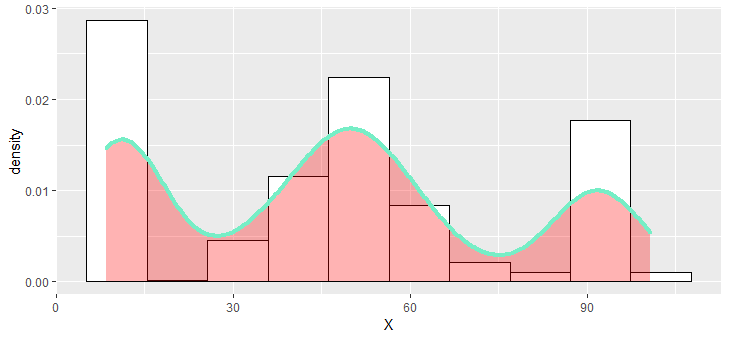
\includegraphics[scale=0.7]{images/good_distrib.png}
	\caption{Mélange gaussien à forte séparation}
\end{figure}
Nous avons lancé l'algorithme EM en choisissant un nombre d'itération $k = 10$. Comme on peut le voir sur la capture d'écran ci-dessous, les paramètres estimés par l'algorithme EM sont assez proche de ceux théoriques.
\begin{figure}[H]
	\centering
	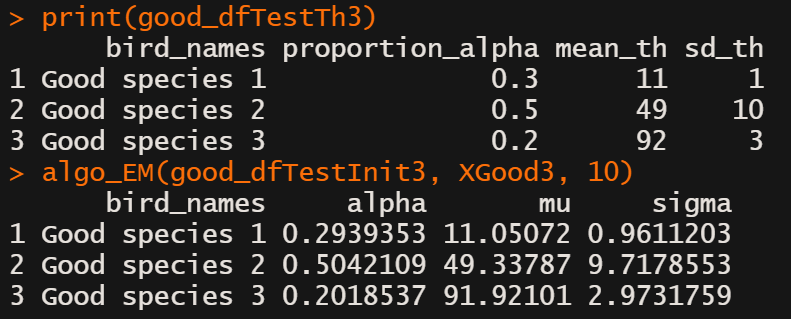
\includegraphics[scale=0.7]{images/EM_good.png}
	\caption{Paramètres théoriques VS paramètres estimés}
\end{figure}

Nous allons maintenant regarder si l'augmentation de la taille de l'échantillon du mélange gaussien avec "fortes séparations" aura pour effet de diminuer l'erreur absolue entre les paramètres estimés par l'algorithme EM et les valeurs théoriques. Pour cela nous allons utiliser notre fonction \textit{Monte-Carlo}.

\begin{lstlisting}
	Monte_Carlo = function(data_th, data_init, k, n, N){
		J = dim(data_th)[1]
		df_MonteCarlo = data.frame()
		iteration = c()
		for(i in 1:k){
			X = simulation(data_th, n)
			data_EM = algo_EM(data_init, X, N)
			df_error = calcul_error(data_th, data_EM)
			df_MonteCarlo = rbind((df_MonteCarlo), df_error)
			v_iter = rep(paste("itération",i,sep="_"), J)
			iteration = append(iteration, v_iter)
		}
		df_MonteCarlo = cbind(iteration, df_MonteCarlo)
		return(df_MonteCarlo)
	}
\end{lstlisting}

Le principe de fonctionnement de cette dernière est le suivant: \\
Pour une taille d'échantillon $n$ fixée, nous exécutons $k$ fois l'algorithme EM pour des échantillons différents. À partir de cela, nous calculons les $3 \times 3 \times K$ erreurs absolues entre les paramètres estimés par l'algorithme EM et les paramètres théoriques. Cette fonction prend donc en arguments :
\begin{itemize}
	\item data\_t,h le dataframe contenant les paramètres $\alpha$, $\mu$ et $\sigma$ théoriques \\
	\item data\_init, le dataframe contenant les paramètres ($\alpha$, $\mu$, $\sigma$) initialement choisis \\
	\item $k$, le nombre d'échantillons que l'on souhaite générer aléatoirement \\
	\item $n$ la taille des échantillons (les k échantillons seront de tailles n), et \\
	\item $N$, le nombre d'itérations de l'algorithme EM
\end{itemize}

Elle retourne un dataframe contenant les erreurs absolues de chaque paramètres des $k$ échantillons de Monte Carlo.

Nous avons effectué 100 itérations de Monte-Carlo pour les différentes tailles d'échantillons suivantes:
\begin{itemize}
	\item $n = 100$ \\
	\item $n = 250$ \\
	\item $n = 500$
\end{itemize}

Les boites à moustaches (boxplot) ci-dessous, représentent l'erreur absolue entre les paramètres estimés par l'algorithme EM et ceux théoriques.

\begin{figure}[H]
	\centering
	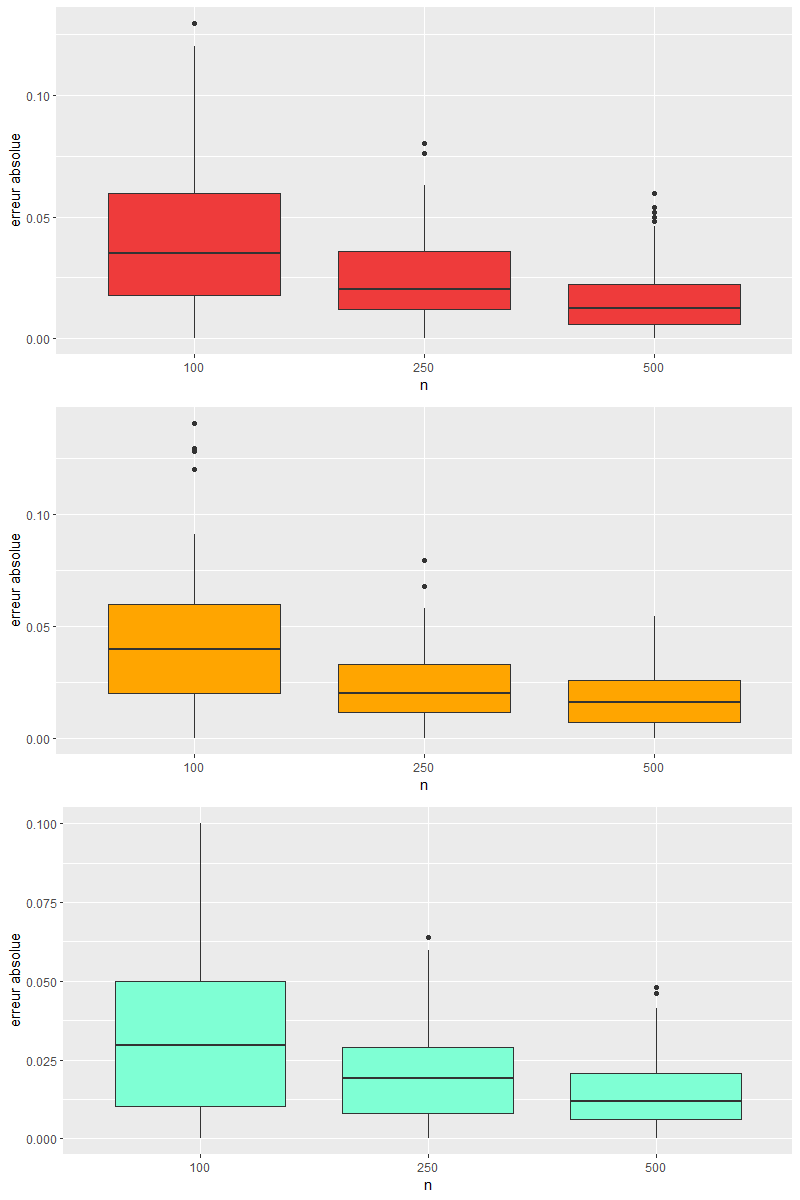
\includegraphics[scale=0.5]{images/good_alpha.png}
	\caption{Boxplot des erreurs absolues pour $\alpha_1$, $\alpha_2$ et $\alpha_3$}
\end{figure}

\begin{figure}[H]
	\centering
	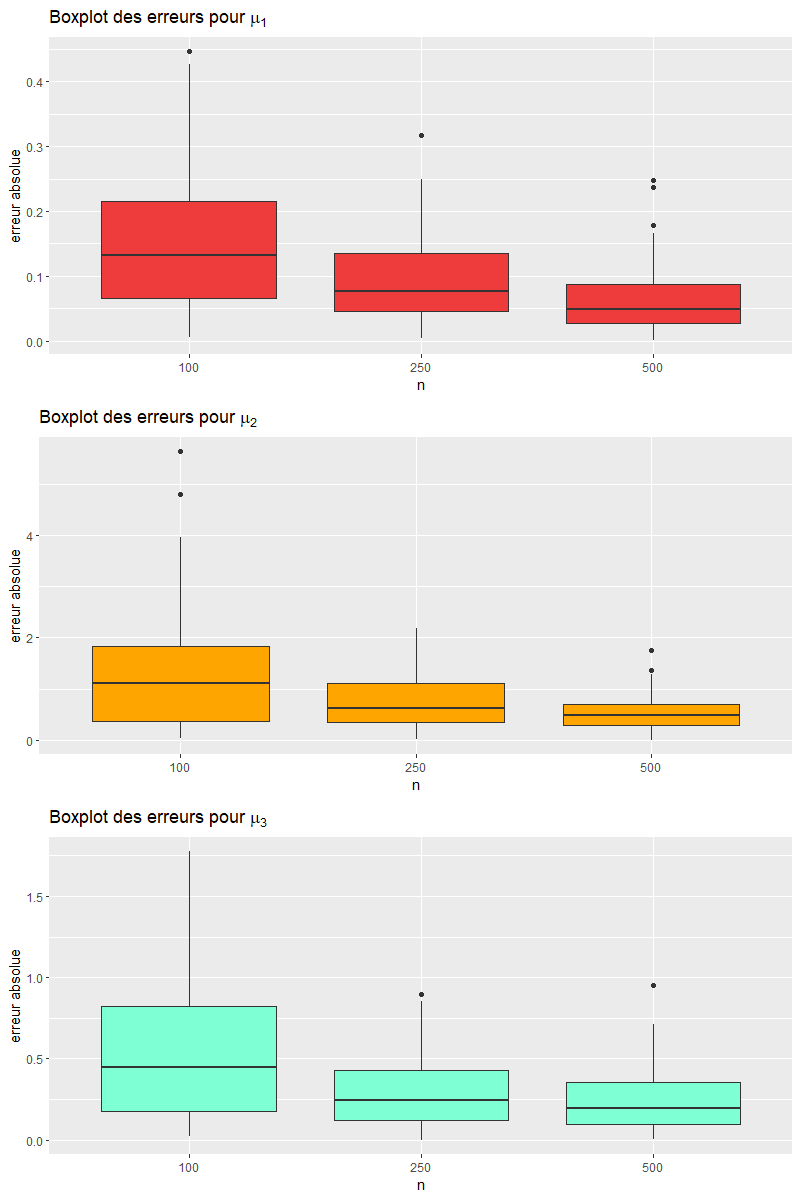
\includegraphics[scale=0.5]{images/good_mu.png}
	\caption{Boxplot des erreurs absolues pour $\mu_1$, $\mu_2$ et $\mu_3$}
\end{figure}
D'après les boites à moustaches, nous constatons que plus la taille de l'échantillons du mélange gaussien est grande, plus l'erreur absolue entre les paramètre estimés par l'algorithme EM et ceux théoriques diminuent.


\subsection{Étude d'un mélange gaussien à faible séparations}
Dans cette partie, nous nous intéresserons à un mélange de trois lois gaussiennes ayant comme loi respectives $\mathcal{N}(\mu_1, \sigma_1)$, $\mathcal{N}(\mu_2, \sigma_2)$ et $\mathcal{N}(\mu_3, \sigma_3)$ faiblement séparées, c'est à dire avec des paramètres assez proches les uns des autres (\underline{i.e.} $|\alpha_i$ - $\alpha_j|_{i \neq j}$; $|\mu_i$ - $\mu_j|_{i \neq j}$; $|\sigma_i$ - $\sigma_j|_{i \neq j}$ assez petits).
De même que pour la première étude, nous avons généré un échantillon d'un mélange de trois lois gaussiennes de taille 500, cette fois-ci avec faible séparation. Les trois lois du mélange sont les suivantes:
\begin{itemize}
	\item $\mathcal{N}(5, 1)$
	\item $\mathcal{N}(13.6, 11)$
	\item $\mathcal{N}(15.3, 6)$
\end{itemize}
La figure ci-dessous représente la distribution du mélange à faibles séparations;

\begin{figure}[H]
	\centering
	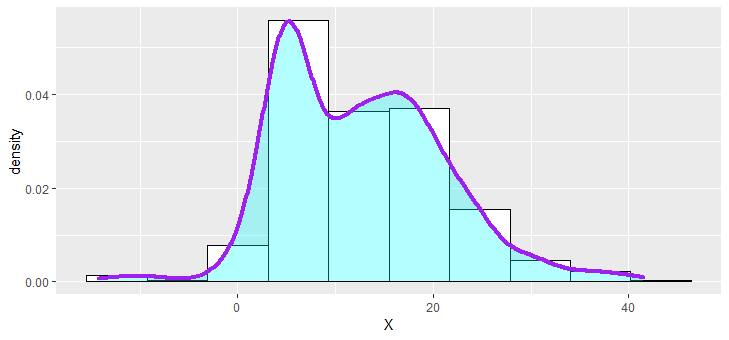
\includegraphics[scale=0.7]{images/bad_distrib.png}
	\caption{Mélange gaussien à faibles séparations}
\end{figure}
Ici aussi, nous avons lancé l'algorithme EM en choisissant un nombre d'itération $k = 10$. Comme nous pouvons le voir sur la capture d'écran ci-dessous, même avec un mélange à faibles séparations, les paramètres estimés par l'algorithme EM sont assez proches de ceux théorique.
\begin{figure}[H]%
	\centering
	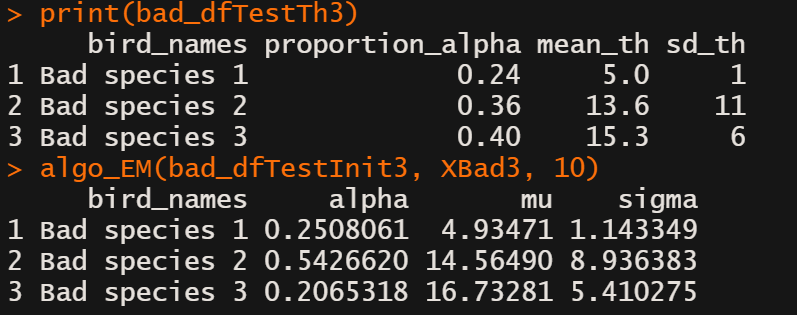
\includegraphics[scale=0.7]{images/EM_bad.png}
	\caption{Paramètres théoriques VS paramètres estimés}
\end{figure}

De même que pour l'étude précèdente, nous allons maintenant regarder si l'augmentation de la taille de l'échantillon du mélange gaussien généré aléatoirement aura pour effet de diminuer l'erreur absolue entre les paramètres estimés par l'algorithme EM et les valeurs théoriques dans le cas d'un mélange à faibles séparations. Pour cela nous allons utiliser notre fonction \textit{Monte-Carlo}. \\
Nous avons effectué 100 itérations de Monte-Carlo pour les différentes tailles d'échantillons suivantes:
\begin{itemize}
	\item $n = 100$ \\
	\item $n = 250$ \\
	\item $n = 500$
\end{itemize}
Les boites à moustaches (boxplot) ci-dessous, modélisent l'erreur absolue entre les paramètres estimés par l'algorithme EM et ceux théoriques dans le cas d'une faible séparation.
\begin{figure}[H]
	\centering
	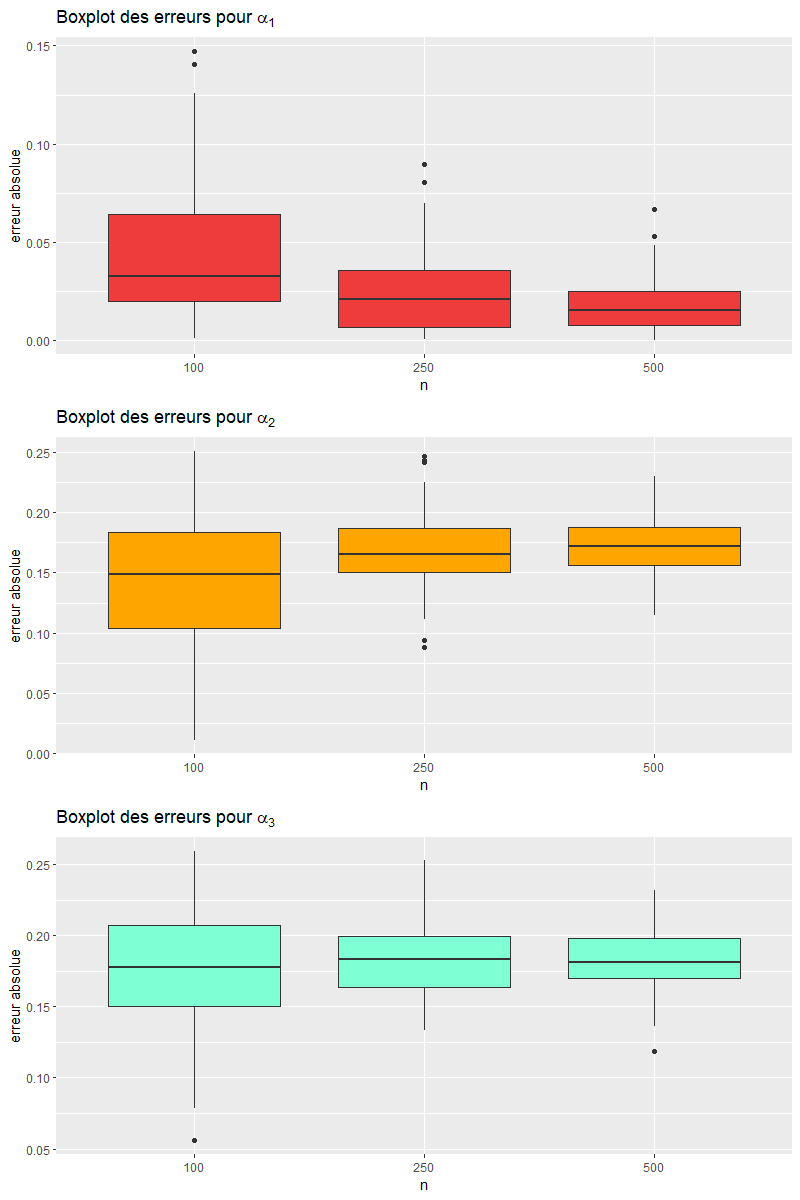
\includegraphics[scale=0.5]{images/bad_alpha.png}
	\caption{Boxplot des erreurs absolues pour $\alpha_1$, $\alpha_2$ et $\alpha_3$}
\end{figure}

\begin{figure}[H]
	\centering
	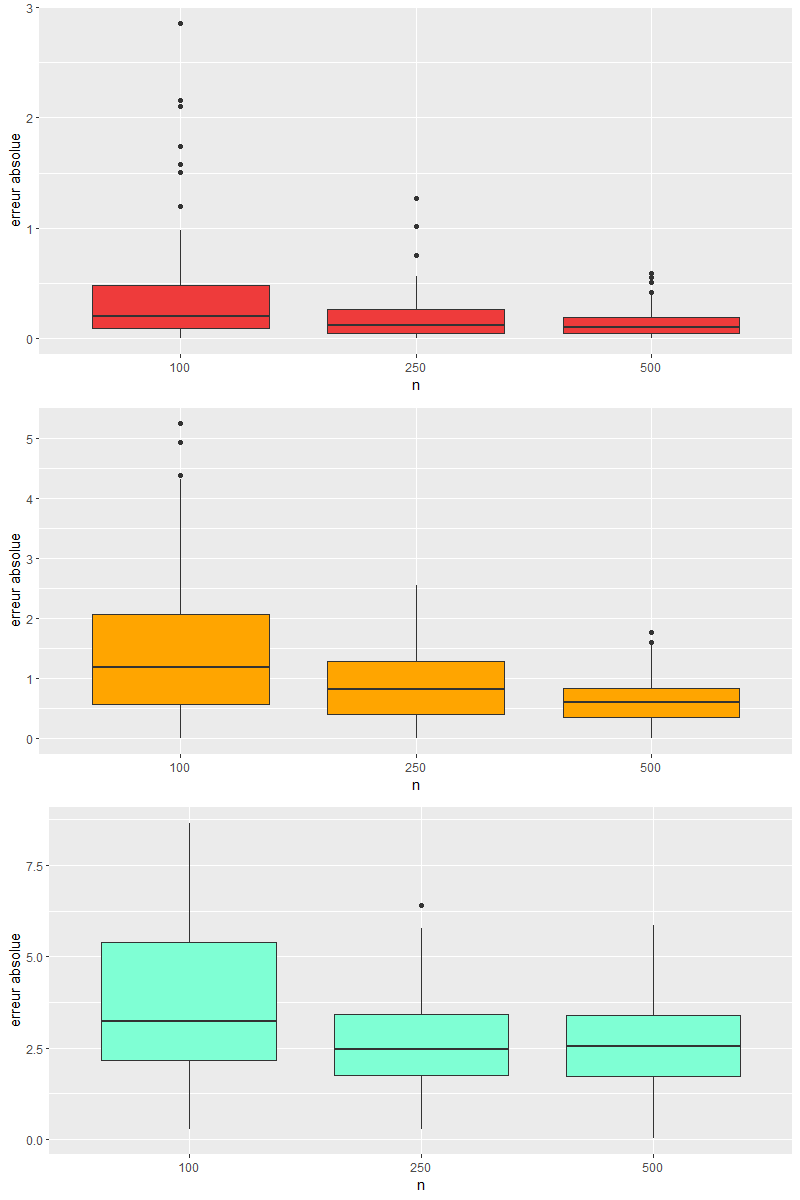
\includegraphics[scale=0.5]{images/bad_mu.png}
	\caption{Boxplot des erreurs absolues pour $\mu_1$, $\mu_2$ et $\mu_3$}
\end{figure}
Même dans le cas d'un mélange à variables faiblement séparées, on constate que plus on augmente la taille de l'échantillons et plus l'erreur absolue diminue, ce qui est rassurant.



\chapter{Un modèle pour les nids d'oiseaux}

Dans ce quatrième et dernier chapitre, nous nous proposons de mettre en oeuvre ce que nous avons développé dans les précédents chapitres. Nous allons nous placer en situation réelle, et étudier un jeu de données correspondant à un mélange de lois gaussiennes. Notre thématique ne changera pas, il sera toujours question de nids d'oiseaux. 

% section 1
\section{Préambule}

Nous n'avons hélas pu trouver des jeux de données sur la taille de nids d'oiseaux en libre accès. Toutefois, nous avons récupéré sur le site de l'\textit{Université de Lincoln (Royaume-Uni)} la prébublication [4], contenant des informations fortes utiles sur une douzaine d'espèces d'oiseaux.
En voici un extrait :
\begin{center}
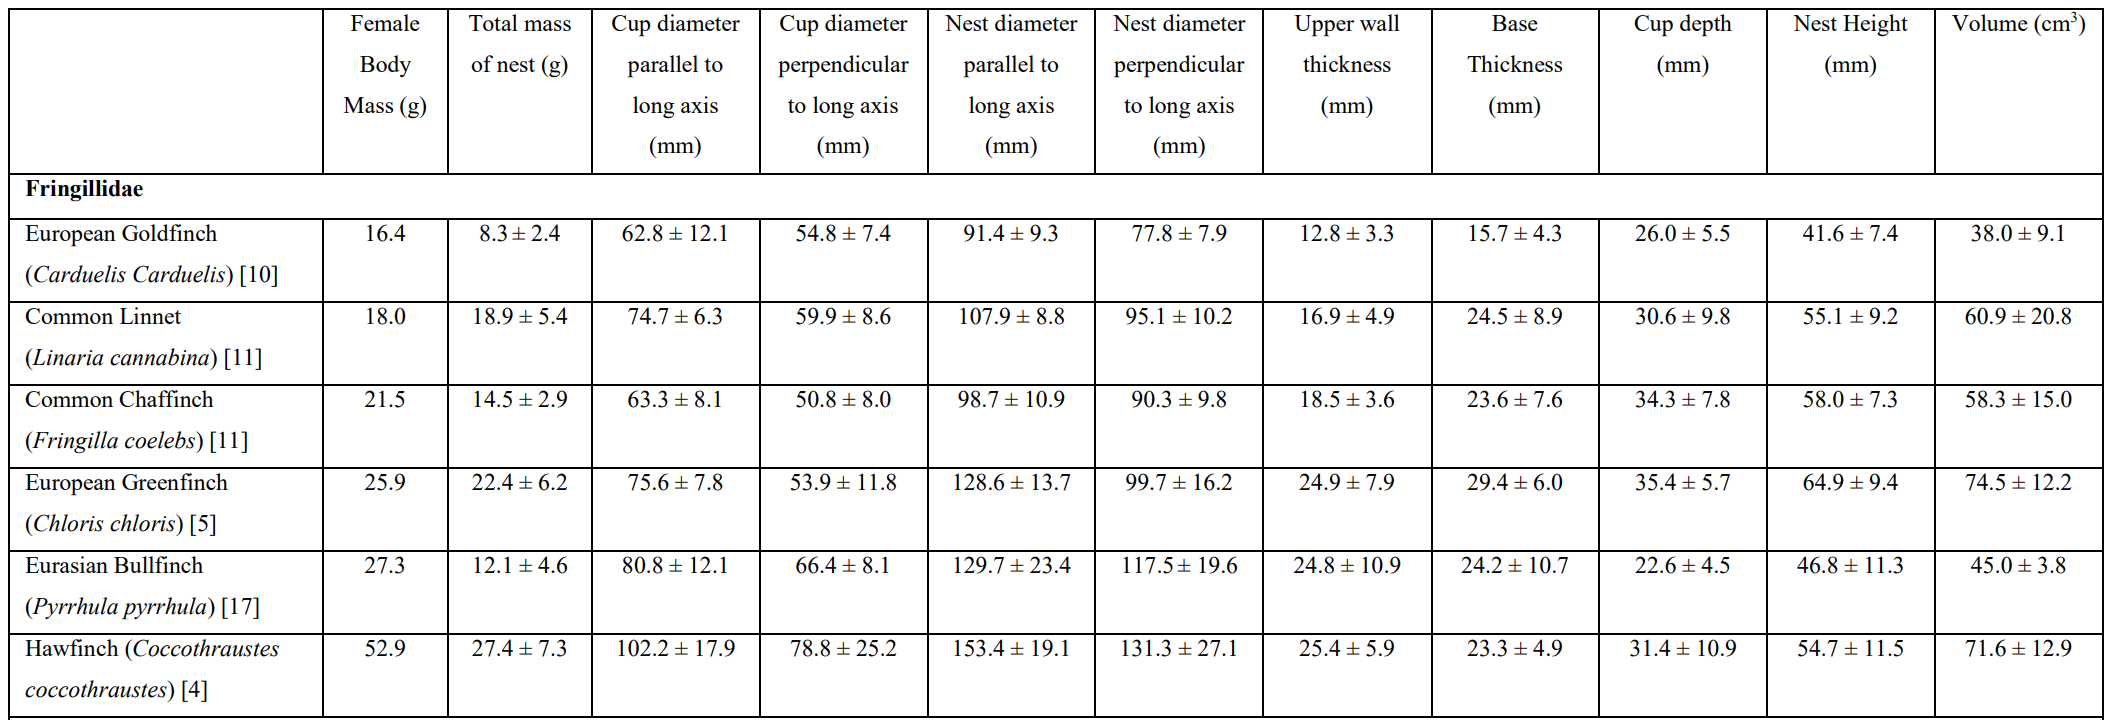
\includegraphics[scale = 0.5]{tab_oiseaux.png}
\end{center}

Parmi elles ce trouve des volumes moyens de nids ainsi que la variance associée. \newline


Afin de se conformer aux hypothèses que nous avons précédemment mentionné, nous supposerons ici que les volumes des nids suivent une loi normale. Nous ferons une dernière hypothèse; nous supposerons le nombre de lois connu lors des observations. \newline

Plaçons nous dès à présent dans le cadre d'une étude. Pour ce faire, commençons par établir une méthodologie. 
Il sera en premier lieu choisi, aléatoirement, plusieurs espèces d'oiseaux parmi celles que nous avons à disposition. Puis nous allons générer, avec \textit{R}, les données dont nous avons besoin. Cet $n$-échantillon sera créé grâce à notre fonction de simulation. Notre jeu de données étant prêt, nous pourrons commencer l'étude. \newline

Le premier problème qui se posera sera celui du choix des paramètres initiaux, notre algorithme nécessitant des valeurs initiales. Nous avons diverses solutions à notre portée.
\begin{itemize}[label=\adfflowerleft]
\item La première est de faire une exploration des données; via une représentation graphique de la densité de l'échantillon. Pour ce faire nous utilisons la fonction pré-implémentée dans \textit{ggplot}. Cette dernière se base sur une méthode d'estimation non-paramétrique, la méthode d'estimation par noyau. Décrivons brièvement son fonctionnement; son étude n'étant pas essentielle dans le cadre de ce projet. C'est une méthode qui estime point par point la densité de l'échantillon, via la fonction $\widehat{f_n}(x)$ définie comme suit

\begin{center}
$
\widehat{f_n}(x) = \displaystyle \frac{1}{n\times h} \sum_{i=1}^n K\Big(\frac{x - X_i}{h}\Big)
$
\end{center}
\underline{où} $h$ est la taille de la fenêtre et $n$ la taille de l'échantillon. Il s'agit, en quelque sorte, d'une moyenne "locale" en $x$ avec les points de l'échantillon $X_i$ qui appartiennent à la fenêtre $[x-h, x+h]$. $K$ est une fonction de noyau. Souvent, elle est choisie comme une densité gaussienne centrée réduite.

Nous pourrons dès lors récupérer des informations bien utiles; si des pics bien distincts se présentent, cela nous permettra de régler judicieusement les moyennes et variances initiales. Nous détaillerons ceci ultérieurement. \newline
\item Une seconde solution est d'utiliser est d'utiliser les quantiles pour l'estimation des moyennes, et l'écart-type empirique pour les variances initiales. Nous détaillerons également cela lors de l'étude.
\end{itemize}

Une fois cela fait, nous pourrons exécuter notre algorithme et obtenir son estimation des paramètres. Nous pourrons dès lors émettre les conclusions appropriées.\newline
Nous partons, pour ainsi dire, à l'aveugle, mais il sera gardé en mémoire les vraies valeurs, afin de vérifier si nous avons abouti aux bonnes conclusions. \newline
Nous avons, à partir du tableau de données sus-mentionné, construit le data-frame \textit{nest$\_$data} reprenant les noms des espèces, ainsi que les volumes moyens et variances associées. Ce dernier nous servira à créer les échantillons.
\newpage
% section 2
\section{Etude d'un mélange à deux lois}
Dans cette section, nous allons étudier le cas d'un mélange de deux lois. Commençons par sélectionner aléatoirement deux espèces, ainsi que les proportions associées. Pour ce faire, nous utiliserons notre fonction, la fonction \textit{random$\_$species}. 

\begin{lstlisting}
df <- random_species(nest_data, 2)
\end{lstlisting}

Nous pouvons dès lors générer l'échantillon, à l'aide de notre fonction \textit{simulation}.

\begin{lstlisting}
data <- simulation(df, 500)
\end{lstlisting}

Nous commençons par tracer la courbe de densité associée à l'échantillon.
\begin{center}
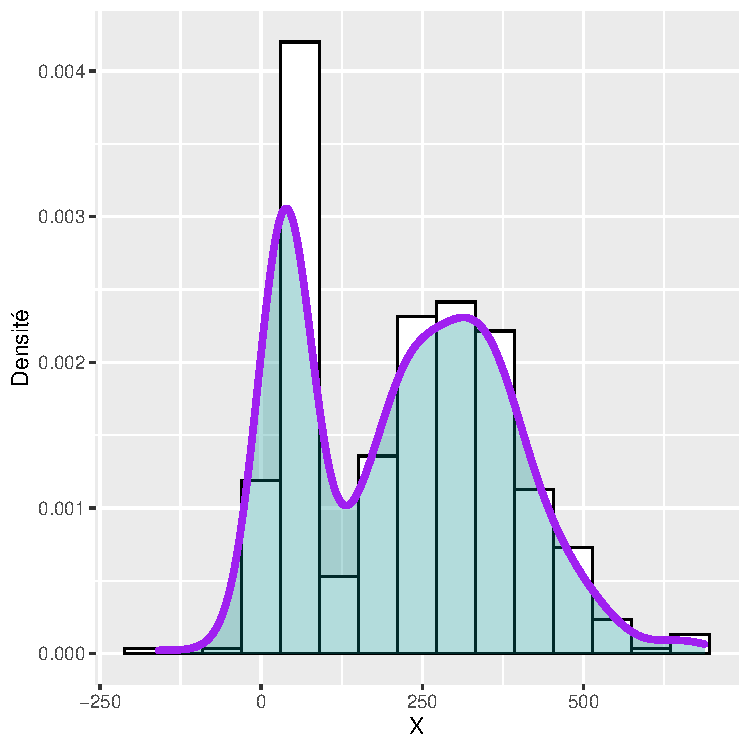
\includegraphics[scale=0.8]{dens_1.pdf}
\end{center}
Le mélange des deux lois se distingue au premier coup d'oeil; nous distinguons nettement deux pics. L'"étalement" des pics n'étant pas les mêmes, nous pouvons supposer sans craintes que les variances des deux lois sont différentes. Il est cependant difficile d'émettre des hypothèses quant aux proportions.\newline
Nous proposon dans ce qui suit deux sous-sections. Dans la première, nous déterminerons les paramètres initiaux via la première méthode décrite précedemment. Nous pourrons dès lors réaliser une première exécution de notre implémentation de l'algorithme EM.
Dans la seconde section, nous ferons de même, en considérant cette fois-ci la seconde méthode de détermination des paramètres initiaux.

\subsection{Première réalisation de l'étude}
%%%
\begin{itemize}[label=\adfflowerleft]
%%%
\item
Commençons par déterminer les paramètres initiaux via une méthode graphique. Cette méthode sera basée sur des heuristiques très approximatives, mais nous permettra d'obtenir des valeurs initiales plutôt correctes. \newline
Pour les moyennes, nous considèrerons l'abscisse correspondant au point culminant des pics; et pour les écarts-types $\sigma$, nous tenterons de déterminer la valeur entre la moyenne précédemment déterminée et le point d'inflexion du pic. Après plusieurs essais sur $R$, nous obtenons
\begin{center}
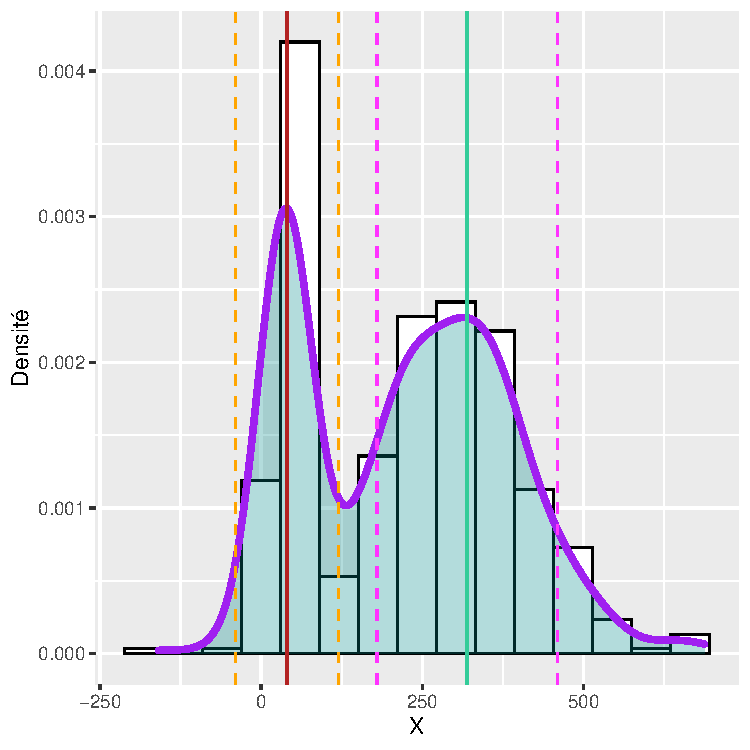
\includegraphics[scale=0.8]{dens_1bis.pdf}
\end{center}
Nous avons tracé des lignes pleines aux abscisses $X=40$ et $X=320$, qui correspondent approximativement au point culminant des pics. Ceci nous donne donc nos moyennes initiales 
\begin{center} 
$\mu_{1_{init}} =  40$ et $\mu_{2_{init}} = 320$. 
\end{center}
Pour les variances, nous avons tracé des lignes en pointillées aux abscisses $\mu_{1_{init}} \pm 80$ et $\mu_{2_{init}} \pm 140$. Nous prendrons donc comme variances initiales 
\begin{center}
$\sigma_{1_{init}} =  80$ et $\sigma_{2_{init}} = 140$
\end{center}
Nous n'avons pas représenté les valeurs des abscisses sur le graphique pour des raisons de lisibilité.\newline
Pour les proportions initiales, nous nous proposons de les prendre égales;  
\begin{center}
$\alpha_{1_{init}}=\alpha_{2_{init}}=0.5$.
\end{center}
Nous pouvons dès lors construire le dataframe des paramètres initiaux;

\begin{lstlisting}
param_init_1 = data.frame(bird_names = c("European Goldfinch", "Ring Ouzel"),
                          alpha_init = c(0.5, 0.5),
                          mean_init = c(40, 320),
                          sd_init = c(80, 140))

\end{lstlisting}

\item Nous avons ainsi tout les éléments nécessaire à l'exécution de notre algorithme. Comme nous l'avons vu dans le précédent chapitre, une dizaine d'itérations suffisent pour obtenir de bons résultats.

\begin{lstlisting}
algo_EM(param_init_1, data, 10)
\end{lstlisting}

\begin{verbatim}
          bird_names     alpha        mu      sigma
1 European Goldfinch 0.2910832  37.76285   9.512478
2         Ring Ouzel 0.7089168 302.51936 125.951894
\end{verbatim}
Nous obtenons ainsi nos paramètres estimés; comparons les avec les valeurs théoriques. Ces dernières sont contenues dans le dataframe \textit{df}. Affichons le :
\begin{verbatim}
         bird_names2 proportion_alpha mean_volume sd_volume
1 European Goldfinch         0.2878713       38.0       9.1
12         Ring Ouzel        0.7121287      298.6     125.1
\end{verbatim}

Les proportions sont toutes deux très bien estimées, les erreurs sont de l'ordre de $1\%$.Il en est de même pour les moyennes, les erreurs d'estimations sont de l'ordre de $1\%$, ce qui est plus que satisfaisant. Les variances sont de mêmes très bien estimées.


\subsection{Seconde réalisation de l'étude}

\begin{itemize}[label=\adfflowerleft]

\item La deuxième méthode à notre disposition pour déterminer les paramètres initiaux est d'utiliser le jeu de données en tant que tel. Pour les deux moyennes initiales, nous allons utiliser les quantiles; et plus précisément le premier et le troisième. En travaillant sur \textit{R}, nous pouvons aisément obtenir ces derniers :

\begin{lstlisting}
quantile(data)
\end{lstlisting}


\begin{verbatim}
       0%       25%       50%       75%      100% 
-44.28714  45.15146 235.38743 352.69611 618.65897
\end{verbatim}
Nous obtenons ainsi nos moyennes initiales :
\begin{center} 
$\mu_{1_{init}} =  45.15146$ et $\mu_{2_{init}} = 352.69611$. 
\end{center}

Concernant les écarts-types, nous prendrons des valeurs d'initialisations égales; et nous utiliserons l'écart-type empirique  
\begin{center}
$\widehat{\sigma} := \displaystyle\frac{1}{J}\sqrt{\displaystyle\frac{1}{n}\sum_{i=1}^n(X_i - \bar{X})^2}$
\end{center}
pour déterminer cette valeur. $J$ est le nombre de mélanges et $n$ la taille de l'échantillon. \newline
Ainsi, 
\begin{center}
$\sigma_{1_{init}} = \sigma_{2_{init}} = \widehat{\sigma}$
\end{center}

Une fois de plus, \textit{R} nous permet de calculer cela aisément: 

\begin{lstlisting}
sqrt(var(data))/2
\end{lstlisting}

\begin{verbatim}
80.29425
\end{verbatim}
Ainsi, 
\begin{center}
$\sigma_{1_{init}} = \sigma_{2_{init}} = 80.29425$. \newline
\end{center}
Pour les proportions initiales, nous proposons de nouveau de les prendre égales, ainsi 
\begin{center}
$\alpha_{1_{init}} = \alpha_{2_{init}} = 0.5$
\end{center}
Par suite, nous construisons le dataframe des paramètres initiaux : 
\begin{lstlisting}
param_init_2 = data.frame(bird_names = c("European Goldfinch", "Ring Ouzel"),
                          alpha_init = c(0.5, 0.5),
                          mean_init = c(45.15146, 352.69611),
                          sd_init = c(80.29425, 80.29425))
\end{lstlisting}
%%%
\end{itemize}
%%%

\item Nous exécutons maintenant l'algorithme avec ce deuxième dataframe de paramètres initiaux.
\begin{lstlisting}
algo_EM(param_init_2, data, 10)
\end{lstlisting}

\begin{verbatim}
          bird_names     alpha        mu      sigma
1 European Goldfinch 0.2936202  37.79956   9.690775
2         Ring Ouzel 0.7063798 303.45499 125.198078
\end{verbatim}

Comme pour le cas précédent, comparons les avec les valeurs théoriques. Nous rappelons une fois de plus ces derniers:
\begin{verbatim}
         bird_names2 proportion_alpha mean_volume sd_volume
1 European Goldfinch         0.2878713       38.0       9.1
12         Ring Ouzel        0.7121287      298.6     125.1
\end{verbatim}

Les proportions sont toutes deux très bien estimées, les erreurs sont de l'ordre de $1\%$.Il en est de même pour les moyennes, les erreurs d'estimations sont de l'ordre de $1\%$, , ce qui est formidable. Les variances sont elles aussi remarquablement bien estimées.

\end{itemize}

Les deux méthodes de déterminations des paramètres initiaux nous donnent des résultats très satisfaisant. Le cas étudié est très favorable, le mélange étant, en quelques sortes, à "fortes séparations".








%%%%%%%%%%%%%
%%%%%%%%%%%%%%%%%%%%%%%%%%%%%%%%%%%%%%%%%%%%%%%%%%%%%%%%%%%%%%%%%%%%%%%
\chapter*{Bibliographie}
\addcontentsline{toc}{part}{Bibliographie}
 

[1] Chafai D., Malrieu F. (2018). Recueil de modèles aléatoires, 105-11, \textit{Prépublication}\newline
\url{https://hal.archives-ouvertes.fr/hal-01897577v3}\newline
\break
[2] Frédéric Santos (2015). L’algorithme EM : une courte présentation, \textit{Document de cours}
\newline\url{https://members.loria.fr/moberger/Enseignement/AVR/Exposes/algo-em.pdf} \newline
\break
[3] Michael Collins (1997). The EM algorithm, \textit{Document de cours}\newline
\url{http://faculty.washington.edu/fxia/courses/LING572/EM_collins97.pdf} \newline
\break
[4] Biddle L.E., Broughton R.E., Goodman A.M., Deeming D.C (2018). Composition of Bird Nests is a Species-Specific Characteristic, \textit{Avian Biology Research, Vol 11, 2, 132-153}\newline
\url{https://core.ac.uk/download/pdf/155777956.pdf}\newline % doc des oiseaux
\break
[5] Fraley C., Raftery A.E., Scrucca L., Murphy T.B, Fop M. (2020). Package 'mclust', \textit{Documentation du package mclust}\newline
 \url{https://cran.r-project.org/web/packages/mclust/mclust.pdf} 


%\url{http://www.cmap.polytechnique.fr/~bansaye/CoursTD6.pdf}
%\url{https://www.lpsm.paris/pageperso/rebafka/BookGraphes/algorithme-em.html} \newline

\pagebreak
%%%%%%%%%%%%%%%%%%%%%%%%%%%%%%%%%%%%%%%%%%%%%%%%%%%%%%%%%%%%%%%%%%%%%%%%%%%%%%%%%%%%


\begin{appendices}
\addcontentsline{toc}{chapter}{Annexes}
% Annexe A
\chapter{Le package \textit{mclust}}
Nous avons, dans un élan d'audace, commencé par programmer à la main l'algorithme EM, en nous appuyant sur le pseudo-code explicité en première partie du chapitre II. \newline

Cependant, il existe une librairie \textit{R} - la librairie \textit{mclust} - contenant une implémentation de l'algorithme EM. Notre algorithme étant fonctionnel, nous ne détaillerons pas ici le fonctionnement de ce Package. Il est néanmoins pertinent de l'expérimenter, voire de comparer ces résultats avec ceux notre algorithme. Nous reprendrons ici les mêmes espèces étudiées lors du dernier chapitre; les divers paramètres seront donc conservés, seul l'échantillon généré changera. Nous nous somme appuyer sur [5] afin d'obtenir les éléments nécessaire à l'utilisation de ce package.

Pour commencer, installons et chargeons le Package \textit{mclust}.
\begin{lstlisting}
install.packages("mclust")
library("mclust")
\end{lstlisting}
%
Nous reprenons les données des nids d'oiseaux :
\begin{lstlisting}
bird_names = c("European Goldfinch", "Common Linnet", "Common Chaffinch",
               "European Greenfinch", "Eurasian Bullfinch", "Hawfinch",
               "Stonechat", "European Robin", "Whinchat", "Song Thrush",
               "Common Blackbird", "Ring Ouzel", "Mistle Thrush")

mean_volume = c(38.0, 60.9, 58.3, 74.5, 45.0, 71.6, 91.0, 68.4, 51.9, 288.9,
                293.6, 298.6, 266.1)

sd_volume = c(9.1,  20.8, 15.0,  12.2,  3.8,  12.9,  46.5, 29.8, 27.4, 55.9,
              78.5,  125.1,  56.6)
\end{lstlisting}
%
Puis, il suffit de construire des dataframe. Ici, nous considérerons deux mélanges; un mélange à deux lois et un autre à trois lois.
\begin{lstlisting}
df_2= data.frame(bird_names = c("European Goldfinch", "Ring Ouzel")
                          ,proportion_alpha = c(0.3, 0.7), mean = c(38, 298.6),
                          sd = c(9.1, 125.1))

df_3= data.frame(bird_names = c("Common Linnet", "Common Chaffinch", "Hawfinch" )
                          ,proportion_alpha = c(0.6, 0.3, 0.1), mean = c(60.9, 58.3, 71.6),
                          sd = c(20.8, 15.0, 12.9))
\end{lstlisting}
%
Nous reprenons ici notre propre fonction de simulation
\begin{lstlisting}
simulation = function(data_th, n=100)
\end{lstlisting}
%
Les prérequis étant posés, nous simulons un échantillon $X2$ de deux espèces d'oiseaux et un autre $X3$ de trois espèces d'oiseaux :
\begin{lstlisting}
set.seed(1907)
X2 <- simulation(df_2)
X3 <- simulation(df_3)
\end{lstlisting}
%
Le Package \textit{mclust} est des plus complet; les possibilités étant très vastes et hors du cadre de ce projet (notamment les fonctionnalités de clustering), nous regarderons uniquement la fonction qui nous intéresse, à savoir la fonction \textit{densityMclust}. \newline
Cette dernière prend en argument des fonctionnalités pertinentes, comme le nombre de mélanges, mais ne permet pas de régler manuellement des valeurs initiales pour les paramètres à estimer.
%

%%%
\section{Un exemple sur un mélange à deux lois}
Commençons par un executer la fonction \textit{densityMclust} sur notre exemple de mélange à deux lois, contenu dans le dataframe $X2$:
\begin{lstlisting}
est_2 <- densityMclust(X2)
\end{lstlisting}
%
Il est en premier lieu retourné le graphe de la densité du mélange de lois.
\begin{center}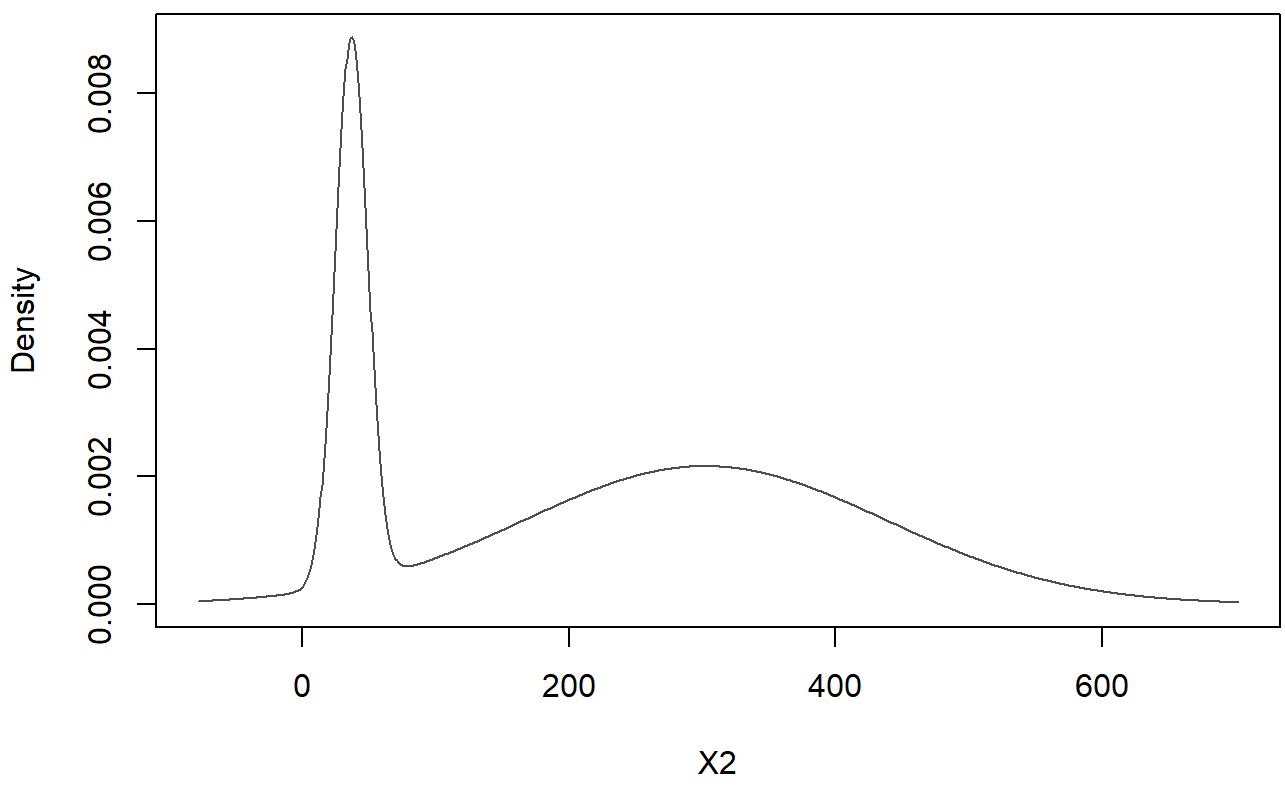
\includegraphics[scale=0.75]{fig1.png}\end{center}
Nous pouvons nettement distinguer les deux "pics", correspondant aux deux gaussiennes mélangées.
Intéressons-nous maintenant à l'objet créé \textit{est$\_$2}.
\begin{lstlisting}
est_2
\end{lstlisting}
\begin{verbatim}
'densityMclust' model object: (V,2) 

Available components: 
 [1] "call"           "data"           "modelName"      "n"              "d"             
 [6] "G"              "BIC"            "loglik"         "df"             "bic"           
[11] "icl"            "hypvol"         "parameters"     "z"              "classification"
[16] "uncertainty"    "density"
\end{verbatim}
%
Ici nous voulons les paramètres estimés, nous nous concentrerons donc que sur la treizième coordonnée de ce vecteur.\newline
Rappelons que les divers paramètres de ce mélange sont : 0.3 et 0.7 en proportions; 38 et 298.6 pour les moyennes; et 9.1 et 125.1 en écart-types.
\begin{lstlisting}
print("Proportions estimées:")
est_2[13]|\$|parameters|\$|pro
print("Moyennes estimées:")
est_2[13]|\$|parameters|\$|mean
print("Ecart-types estimés:")
(est_2[13]|\$|parameters|\$|variance|\$|sigmasq)^(1/2)
\end{lstlisting}
\begin{verbatim}
[1] "Proportions estimées:"
[1] 0.2612243 0.7387757
[1] "Moyennes estimées:"
        1         2 
 36.80898 301.97108 
[1] "Ecart-types estimés:"
[1]  12.16256 136.32256
\end{verbatim}
Ici, le nombre de mélange est exact. Les proportions sont très bien estimées, l'erreur la plus importante est de l'ordre de $4\%$. Il en va de même pour les moyennes, les erreurs sont d'ordres inférieures à $10\%$. Les erreurs sur les variances sont de l'ordre de $10\%$ ou moins, ce qui est plutôt bon. 
\newpage
%%%
\section{Un exemple sur un mélange à trois lois}
Regardons maintenant le cas d'un mélange de trois lois. Afin de mettre à rude épreuve l'algorithme, nous allons choisir les espèces telles que les moyennes et variances soient proches. Les proportions seront quant à elles bien distinctes, nous allons voir pourquoi.
%
\begin{lstlisting}
est_3<- densityMclust(X3)
\end{lstlisting}
\begin{center}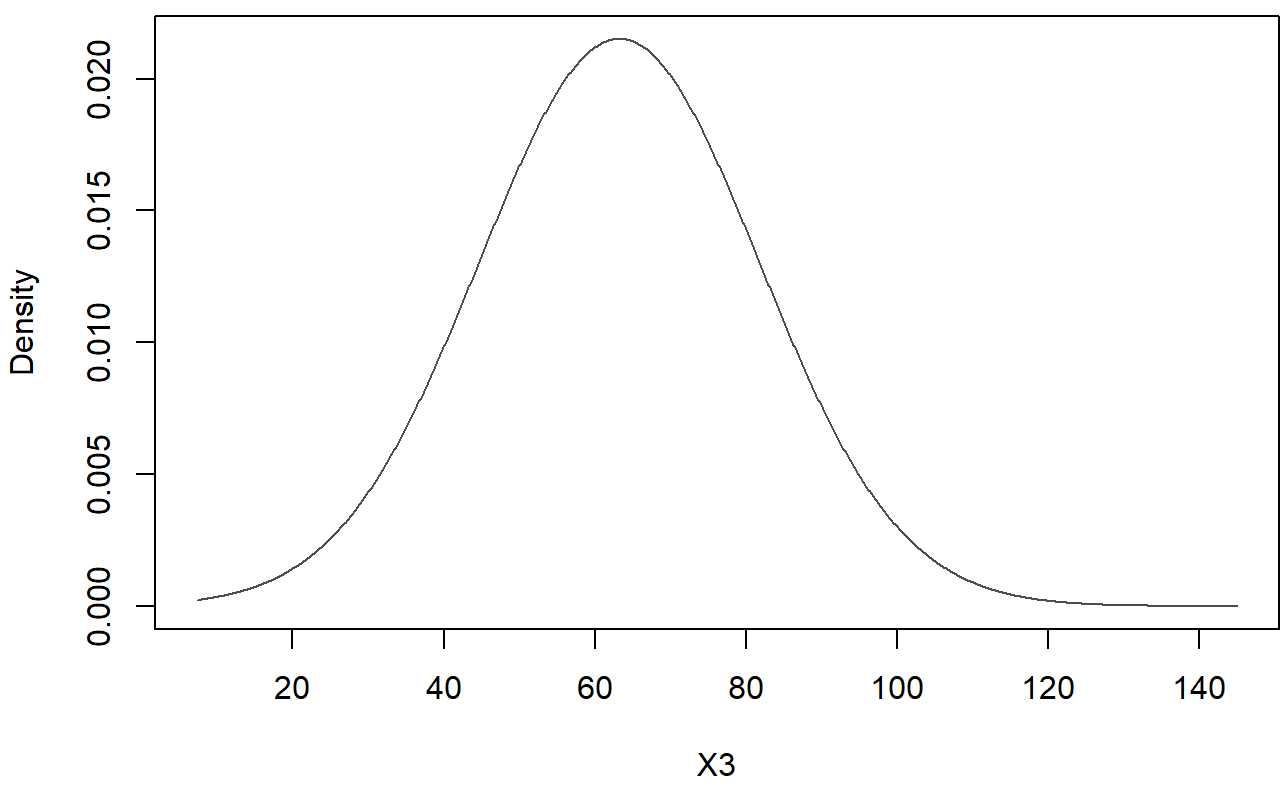
\includegraphics[scale=0.75]{fig2.png}\end{center}
Nous obtenons ici quelque chose d'intéressant; la fonction de densité de ce mélange de trois lois paraît toute à fait gaussienne. Sans une exploration plus approfondie des données, nous commettrions une chagrinante erreur et des conclusions totalement faussées... \newline
%
Il est ici pertinent d'observer la structure des données; plus précisemment, nous allons effectuer un test de \textit{Shapiro}.
\begin{lstlisting}
shapiro.test(X3)
\end{lstlisting}

\begin{verbatim}
	Shapiro-Wilk normality test

data:  X3
W = 0.97982, p-value = 0.1287
\end{verbatim}
La p-value est de 0.1287, ce qui est certes peu élevée, mais pas assez pour rejeter l'hypothèse $(\mathcal{H}_0)$ de normalité. Nous sommes ici dans une situation ambiguë.\newline
%

Observons maintenant comment \textit{densityMclust} se défend fasse à cette situation. \newline
Rappelons que les divers paramètres de ce mélange sont : 0.6, 0.3 et 0.1 en proportions; 60.9, 58.3 et 71.6 en moyenne; et 20.8, 15 et 12.9 en écart-types.
\begin{lstlisting}
print("Proportions estimées:")
est_3[13]|\$|parameters|\$|pro
print("Moyennes estimées:")
est_3[13]|\$|parameters|\$|mean
print("Ecart-types estimés:")
(est_3[13]|\$|parameters|\$|variance|\$|sigmasq)^(1/2)
\end{lstlisting}

\begin{verbatim}
[1] "Proportions estimées:"
[1] 1
[1] "Moyennes estimées:"
[1] 63.20547
[1] "Ecart-types estimés:"
[1] 18.54033
\end{verbatim}
Le premier élément notable est que l'algorithme échoue à établir le nombre correct de lois. L'unique moyenne et écart-type estimés ne sont quant à eux pas absurde. \newline
%
Nous allons relancer la fonction sur le même jeu de données, en précisant cette fois-ci le nombre de lois.
\begin{lstlisting}
est_3b <- densityMclust(X3, G = 3)
print("Proportions estimées:")
est_3b[13]|\$|parameters|\$|pro
print("Moyennes estimées:")
est_3b[13]|\$|parameters|\$|mean
print("Ecart-types estimés:")
(est_3b[13]|\$|parameters|\$|variance|\$|sigmasq)^(1/2)
\end{lstlisting}
\begin{verbatim}
[1] "Proportions estimées:"
[1] 0.2552686 0.5642272 0.1805042
[1] "Moyennes estimées:"
       1        2        3 
56.63179 62.36268 75.13635 
[1] "Ecart-types estimés:"
[1] 17.51051
\end{verbatim}

Les proportions sont plutôt bien estimées, quoique légèrement surestimées pour deux d'entres elles, mais les erreurs restent faibles. Il en est étonnament de même pour les moyennes, qui sont très bien estimées. Les erreurs sont au plus de l'ordre de $5\%$. Ceci est surprenant au vue de l'allure de la densité. Cependant, il n'est estimé qu'un unique écart-type, ce qui n'est guère étonnant. Notons que celui-ci est à peu près égale à la moyenne des écart-types des différentes lois. \newline

Ce cas ambigüe met en exergue les limites de l'algorithme implémenté dans ce package.


\end{appendices}















\end{document}
